\documentclass[12pt]{article}%

%============================================================================
% Assignment Information

\def\assignmentName { Project 3 - Website Analysis                      }
\def\className      { CSE 321: Internet and Web Programming             }
\def\studentName    { Noah Schoonover \\ Myles Willis \\ Adam Schmidt   }
\def\studentEmail   {  }
\def\dueDate        { September 16, 2021                                }
\def\semesterDate   { Fall 2021                                         }

%============================================================================
% Packages

\usepackage{tabularx, makecell}
\usepackage{setspace}
\usepackage[shortlabels]{enumitem}
\renewcommand{\thesubsection}{\thesection.\alph{subsection}}
\usepackage[a4paper, top=2.5cm, bottom=2.5cm, left=1.5cm, right=1.5cm]{geometry}
\usepackage{amsmath, amssymb}
\usepackage{float, graphicx}
\usepackage[bottom]{footmisc}

%============================================================================
% User Defined Commands

\newcommand{\itemAt}[1]{\setcounter{enumi}{#1 - 1}\item}
\newcommand{\ntab}{\hspace*{1cm}}

%============================================================================
% Headers and Document Setup

\doublespacing

%============================================================================
\begin{document}
%============================================================================

%---------------------------------------------------------------------
% Title

\begin{singlespace}
\title{ \assignmentName }
\author{ \studentName \\ {\small \studentEmail} \\ {\it \className}}
\date{\dueDate (\semesterDate)}
\maketitle
\end{singlespace}

%---------------------------------------------------------------------
% Document


\begin{itemize}
    \item Theme:

    The goal of this project is to simplify the way contact information and social accounts are shared with the people you meet.
    we aim to provide users with the ability to share their "Zolink", a personalized contact card web page that can be used for personal,
    business and networking purposes, without the need for their own server or domain. We hope to allow users to share complete
    contact cards with one link, QR code, or Zolink username.

    \item Group Name: Zolink
    \item Group Members:
    \begin{itemize}
        \item Noah Schoonover
        \item Myles Willis
        \item Adam Schmidt
    \end{itemize}
\end{itemize}


\section{Background}

Nearly everyone has accounts on social media platforms such as Instagram, LinkedIn, Snapchat, etc. When you meet someone it can
be a pain to share each of these accounts individually in addition to other contact information. Why not have a way to share the
information you want all at once?


\section{Website Analysis}
    \begin{enumerate}[2.a.]

        \item Five existing websites found which offer services for creating digital contact/ business cards include: CardURL, OVOU Card, Switchit, vCard Maker and HiHello. Each of these sites vary in their execution of this service in their use of the unique features they offer to customers and the way they envision their system being used. The features of each of these sites is listed below.

        \begin{enumerate}
            \item [--] \textbf{CardURL (Paid service subscription)}

            \begin{itemize}
                \item View and download count tracking (card statistics)
                \item Notify contacts of modifications
                \item Create multiple cards with varying information
                \item Direct import to contact lists on mobile devices
                \item Short, personalized URL and QR code
                \item Profile photo
            \end{itemize}

            \item [--] \textbf{OVOU Card (Paid physical card)}


            \begin{itemize}
                \item Physical card with NFC and QR code
                \item Customize-able card and personal page
                \item Add directly to contacts on mobile devices
                \item Host individual URL as public web-page
                \item Choose username or have one generated through OVOU site
                \item Profiles do not show on search engines
            \end{itemize}

            \item [--] \textbf{Switchit (Paid service subscription + App)}

            \begin{itemize}
                \item Add media (Video and Images)
                \item Smart Contact Manager
                \item Fully developed app to create and share profiles
                \item Personalized notes on contacts users receive
                \item Business card scanner (Photo to digital)
                \item Sync with Outlook, Google Calendar, iCloud Calendar
                \item File attachment (PDF fill forms , documents ,etc)
                \item Call and text contacts using the app
            \end{itemize}

            \item [--] \textbf{vCard Maker (Free)}
            \begin{itemize}
                \item Add job/social network information
                \item Lacks QR code
                \item Lacks Unique link/online hosting
                \item (.vcf) file creation and download
                \item Attach .vcf file to emails and messages to be downloaded
            \end{itemize}

            \item [--] \textbf{HiHello (Paid service subscription + App)}

            \begin{itemize}
                \item Mobile app
                \item QR code, NFC tag sharing
                \item Address book
                \item Import google contacts
                \item Paper business card transcriptions
                \item Custom colors/page customization
                \item Personalized link
                \item Include files and profile videos
                \item Sync with Outlook and Google services
            \end{itemize}
        \end{enumerate}

        \item We are aiming to:
        \begin{itemize}
            \item Allow users to create an account and add the information they desire on their Zolink.
            \item Allow users to create multiple contact cards with different purposes.
            \item Have an option to make contact cards public or private.
            \item Create a unique URL and QR code for every card so that the user will be able to share these cards easily.
        \end{itemize}
        \item
    \end{enumerate}

\begin{center}
    \begin{tabular}{|l|l|l|l|l|l|l|}
        \hline
         & Zolink & CardURL & OVOU Card & Switchit & vCard Maker & HiHello \\
         \hline
        QR Code & V & V & V & X & X & V \\
        \hline
        Unique URL & V & V & V & X & X & V \\
        \hline
        Multiple Cards & V & V & X & X & X & X \\
        \hline
        Add personal info & V & X & V & V & V & V \\
        \hline
        Page Customization & V & O & V & O & X & V \\
        \hline
        Import to mobile & X & V & V & V & X & V \\
        \hline
        Physical card & X & X & V & X & X & X \\
        \hline
        File Upload & V & X & X & V & V & V \\
        \hline
        Public/Private cards & V & V & X & V & X & X \\
        \hline
    \end{tabular}
\end{center}

\clearpage
\section{Storyboard}

\begin{enumerate}[a.]
    \item The user-base for Zolink will include nearly any demographic, as almost anyone can make use of a digital business card. Most people have multiple social media accounts as well as email addresses, phone numbers, and a physical address. Simply put, anyone who has the ability to use the web and create an account will find Zolink useful.

    All users will have the same role and capabilities on Zolink, aside from the developers who will be able to moderate user information if needed.

    \item
\end{enumerate}

\begin{center}
    {\bf \Large Welcome Page}
    \makebox[\textwidth]{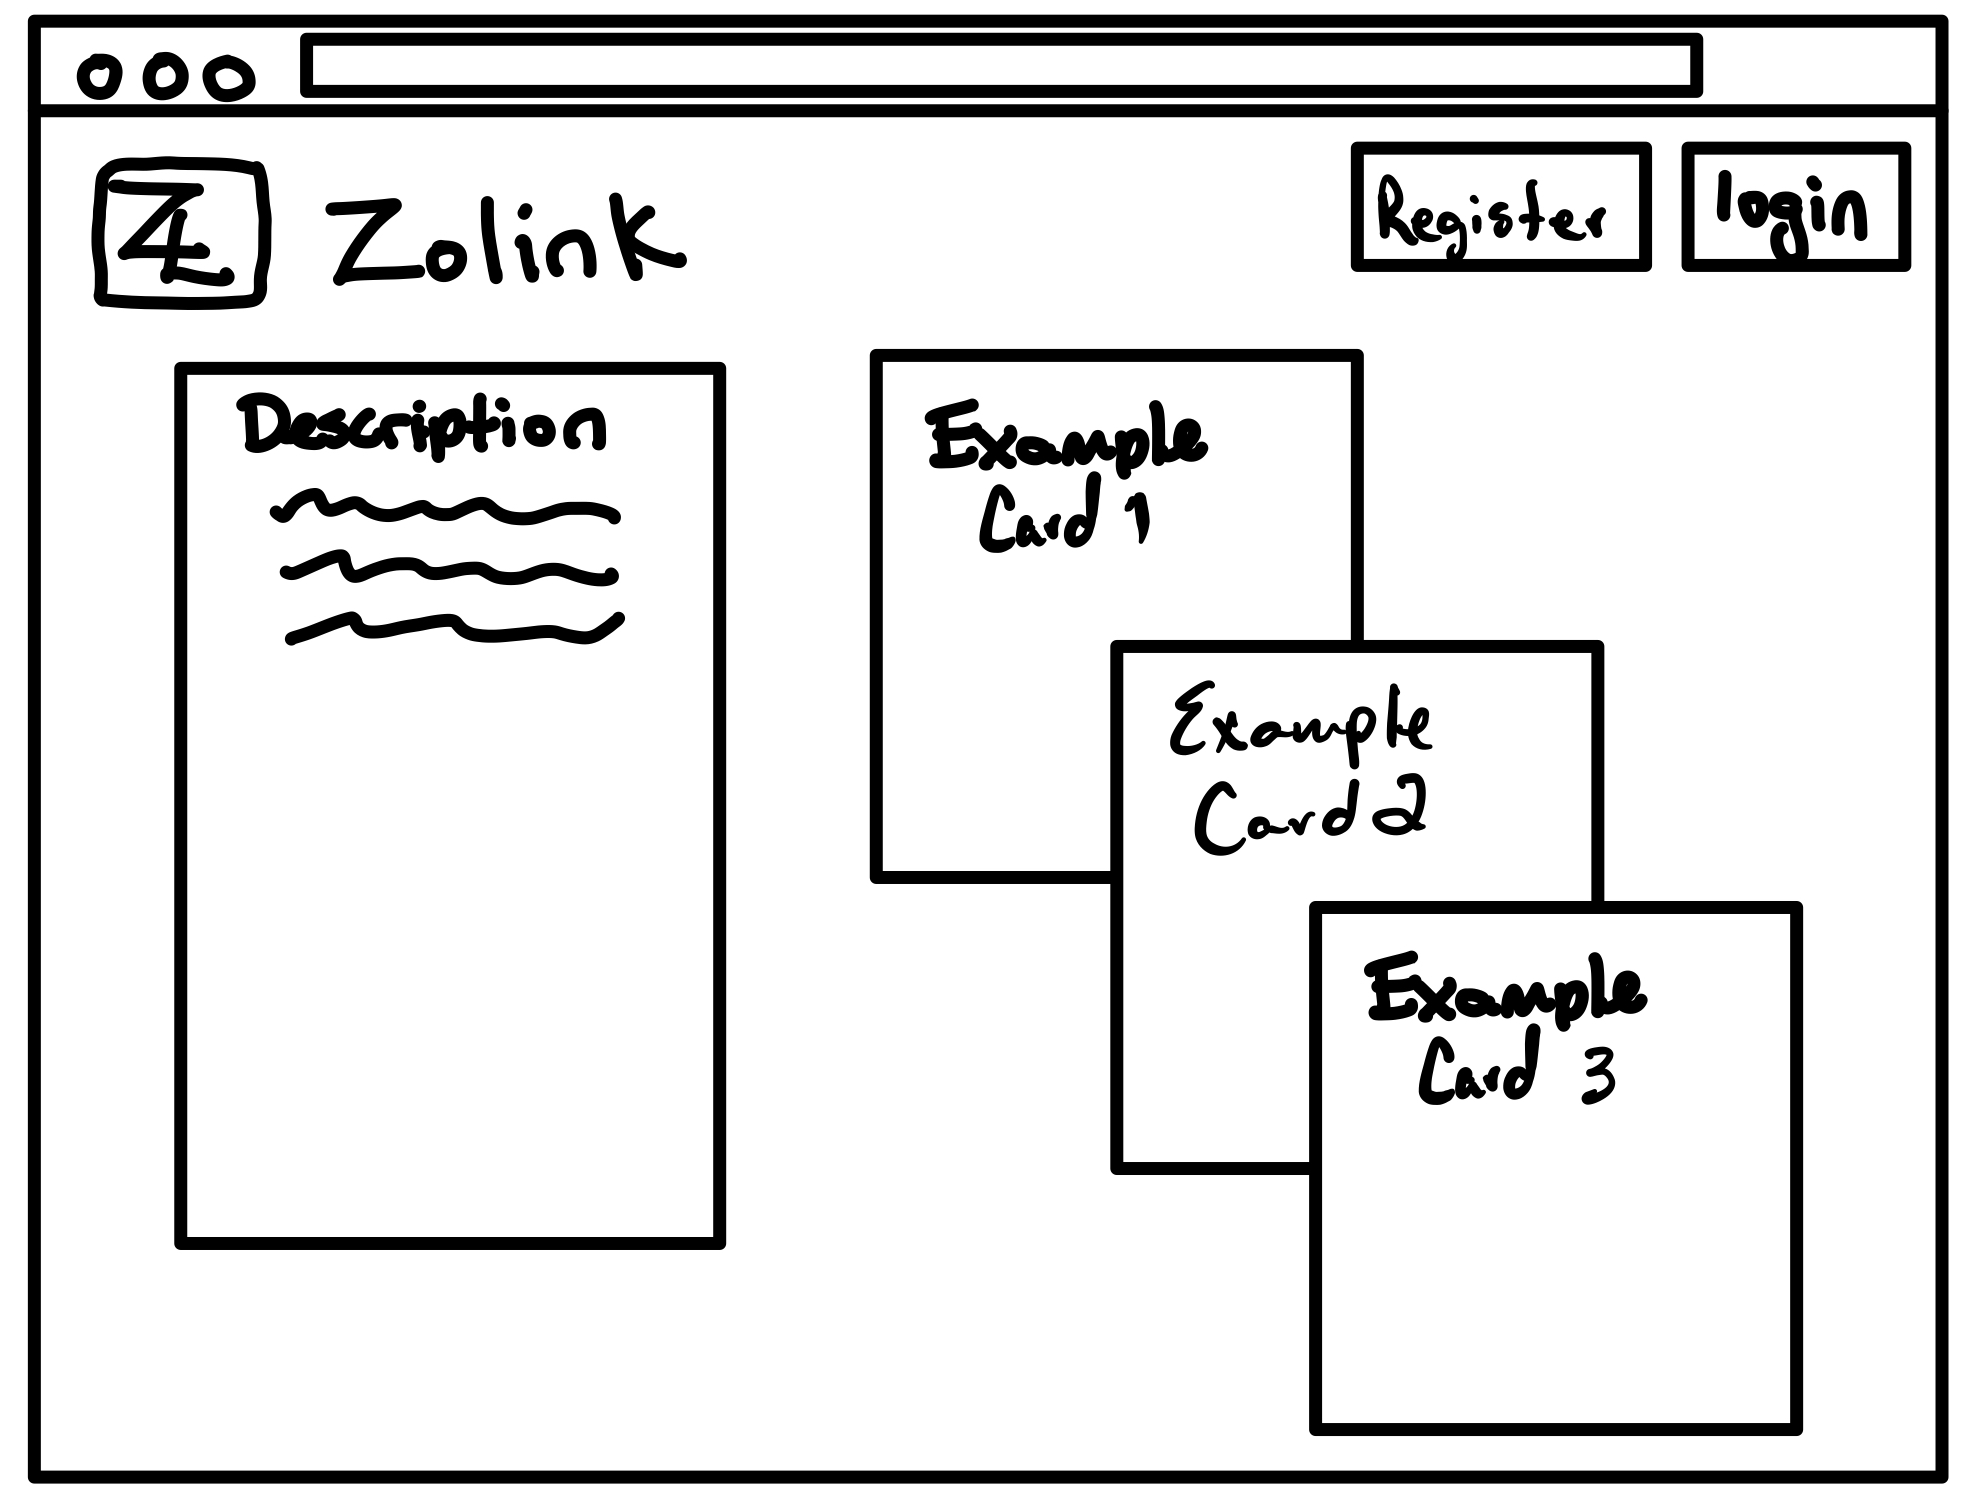
\includegraphics[width=0.98\paperwidth]{storyboard_images/welcome_page.jpeg}}
    {\it This page will provide an explanation of Zolink's purpose and show a few example cards.}

    \clearpage
    {\bf \Large Account Creation Page}
    \makebox[\textwidth]{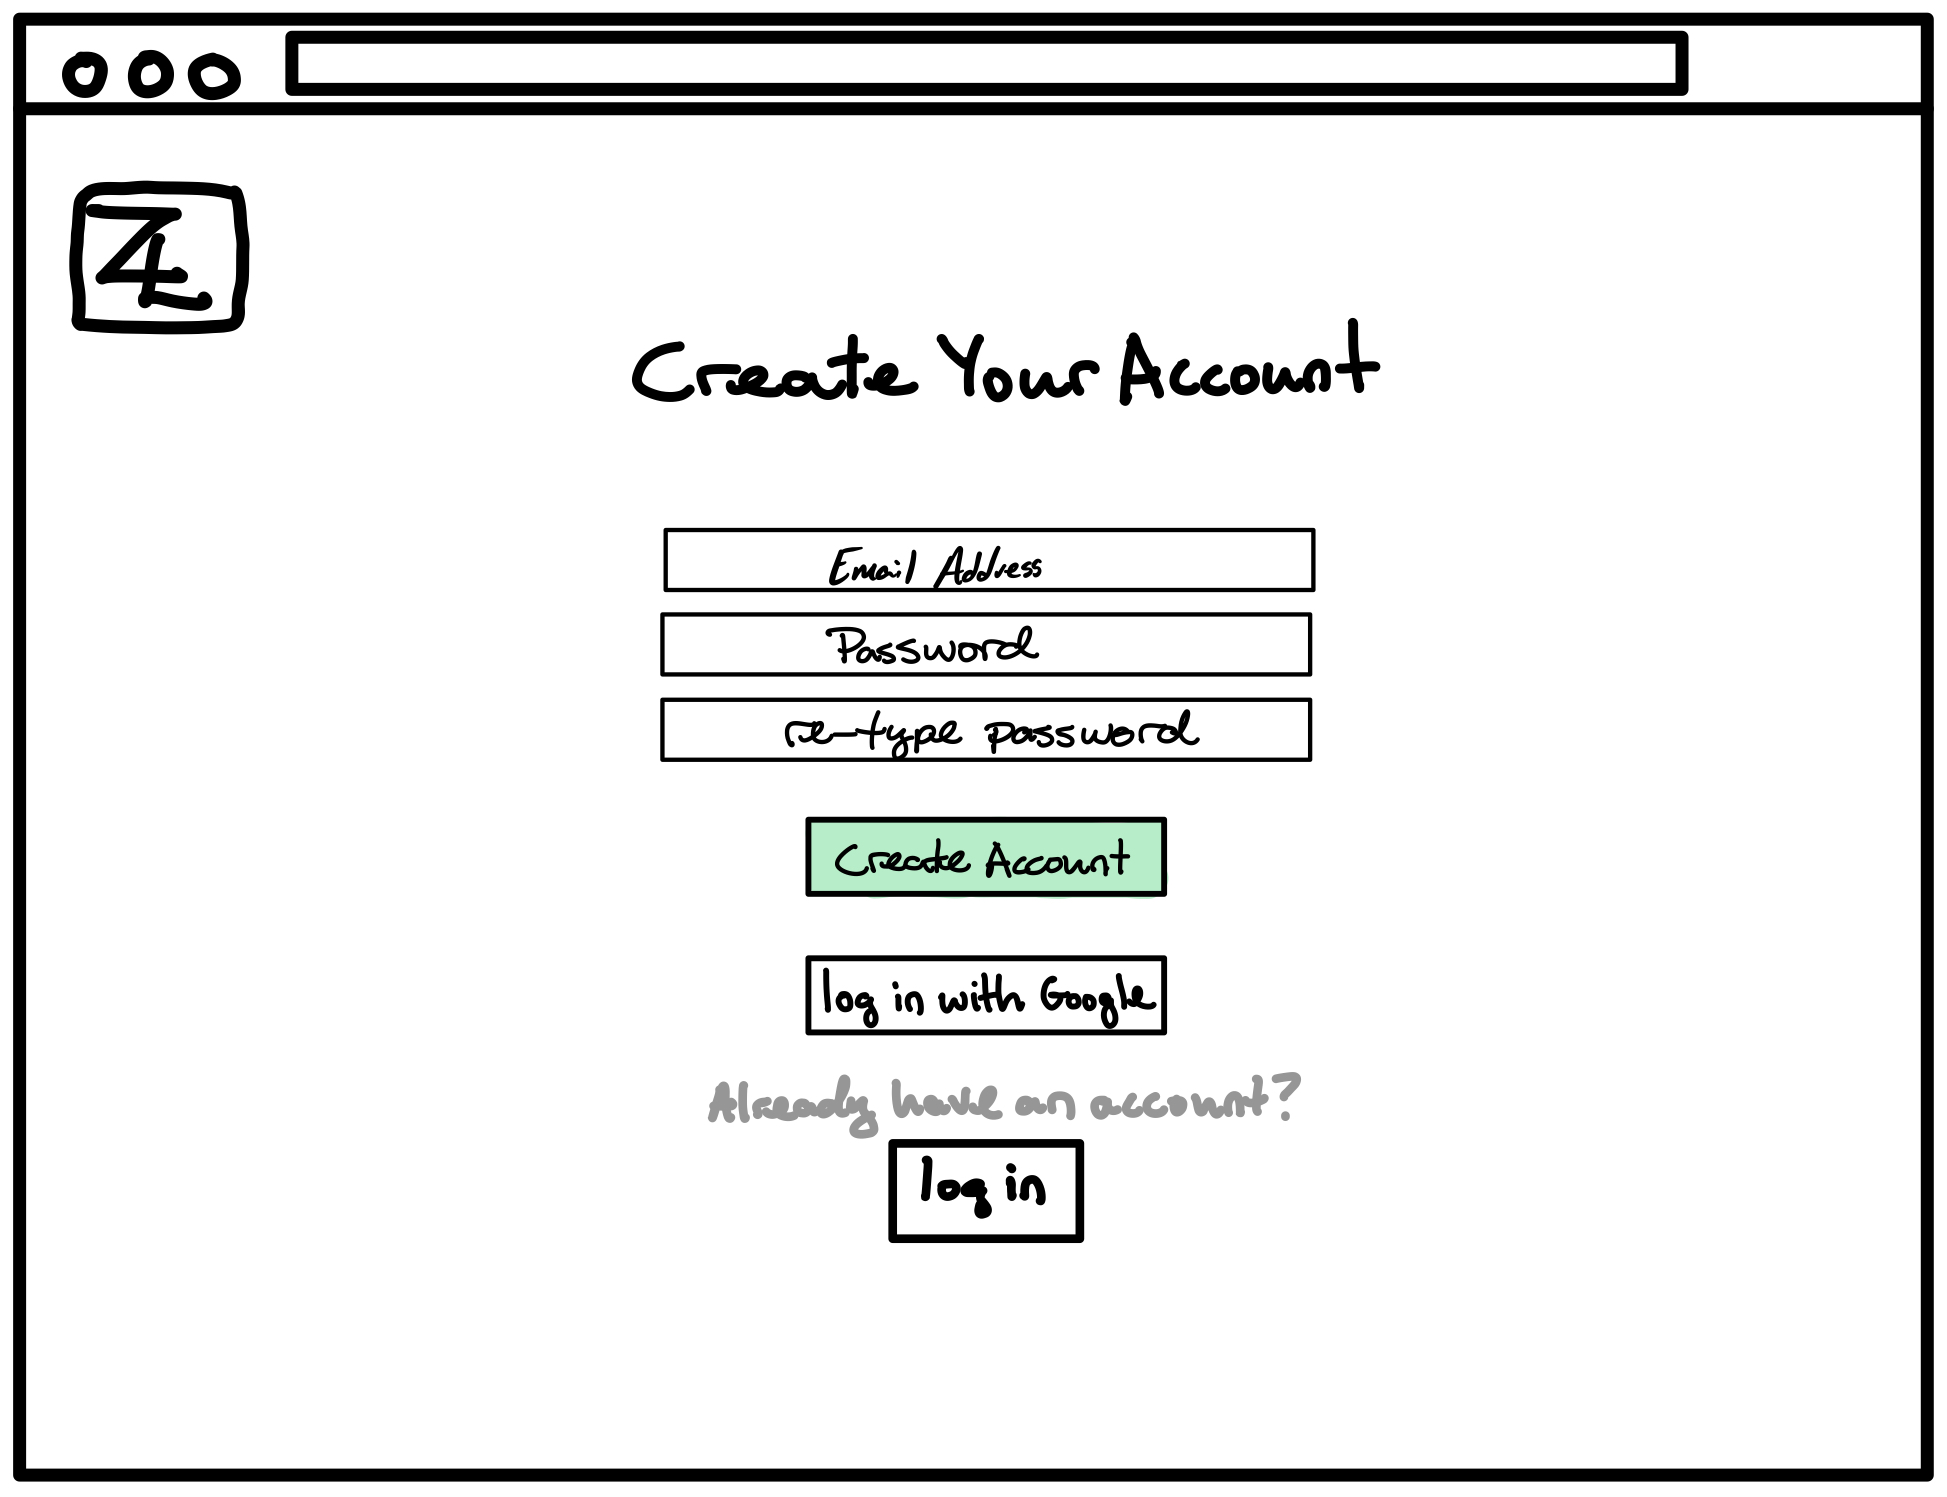
\includegraphics[width=0.98\paperwidth]{storyboard_images/account_creation.jpeg}}
    {\it NOTE: It is to be determined whether the Google login API will be included.}

    \clearpage
    {\bf \Large Card List Page (New Account)}
    \makebox[\textwidth]{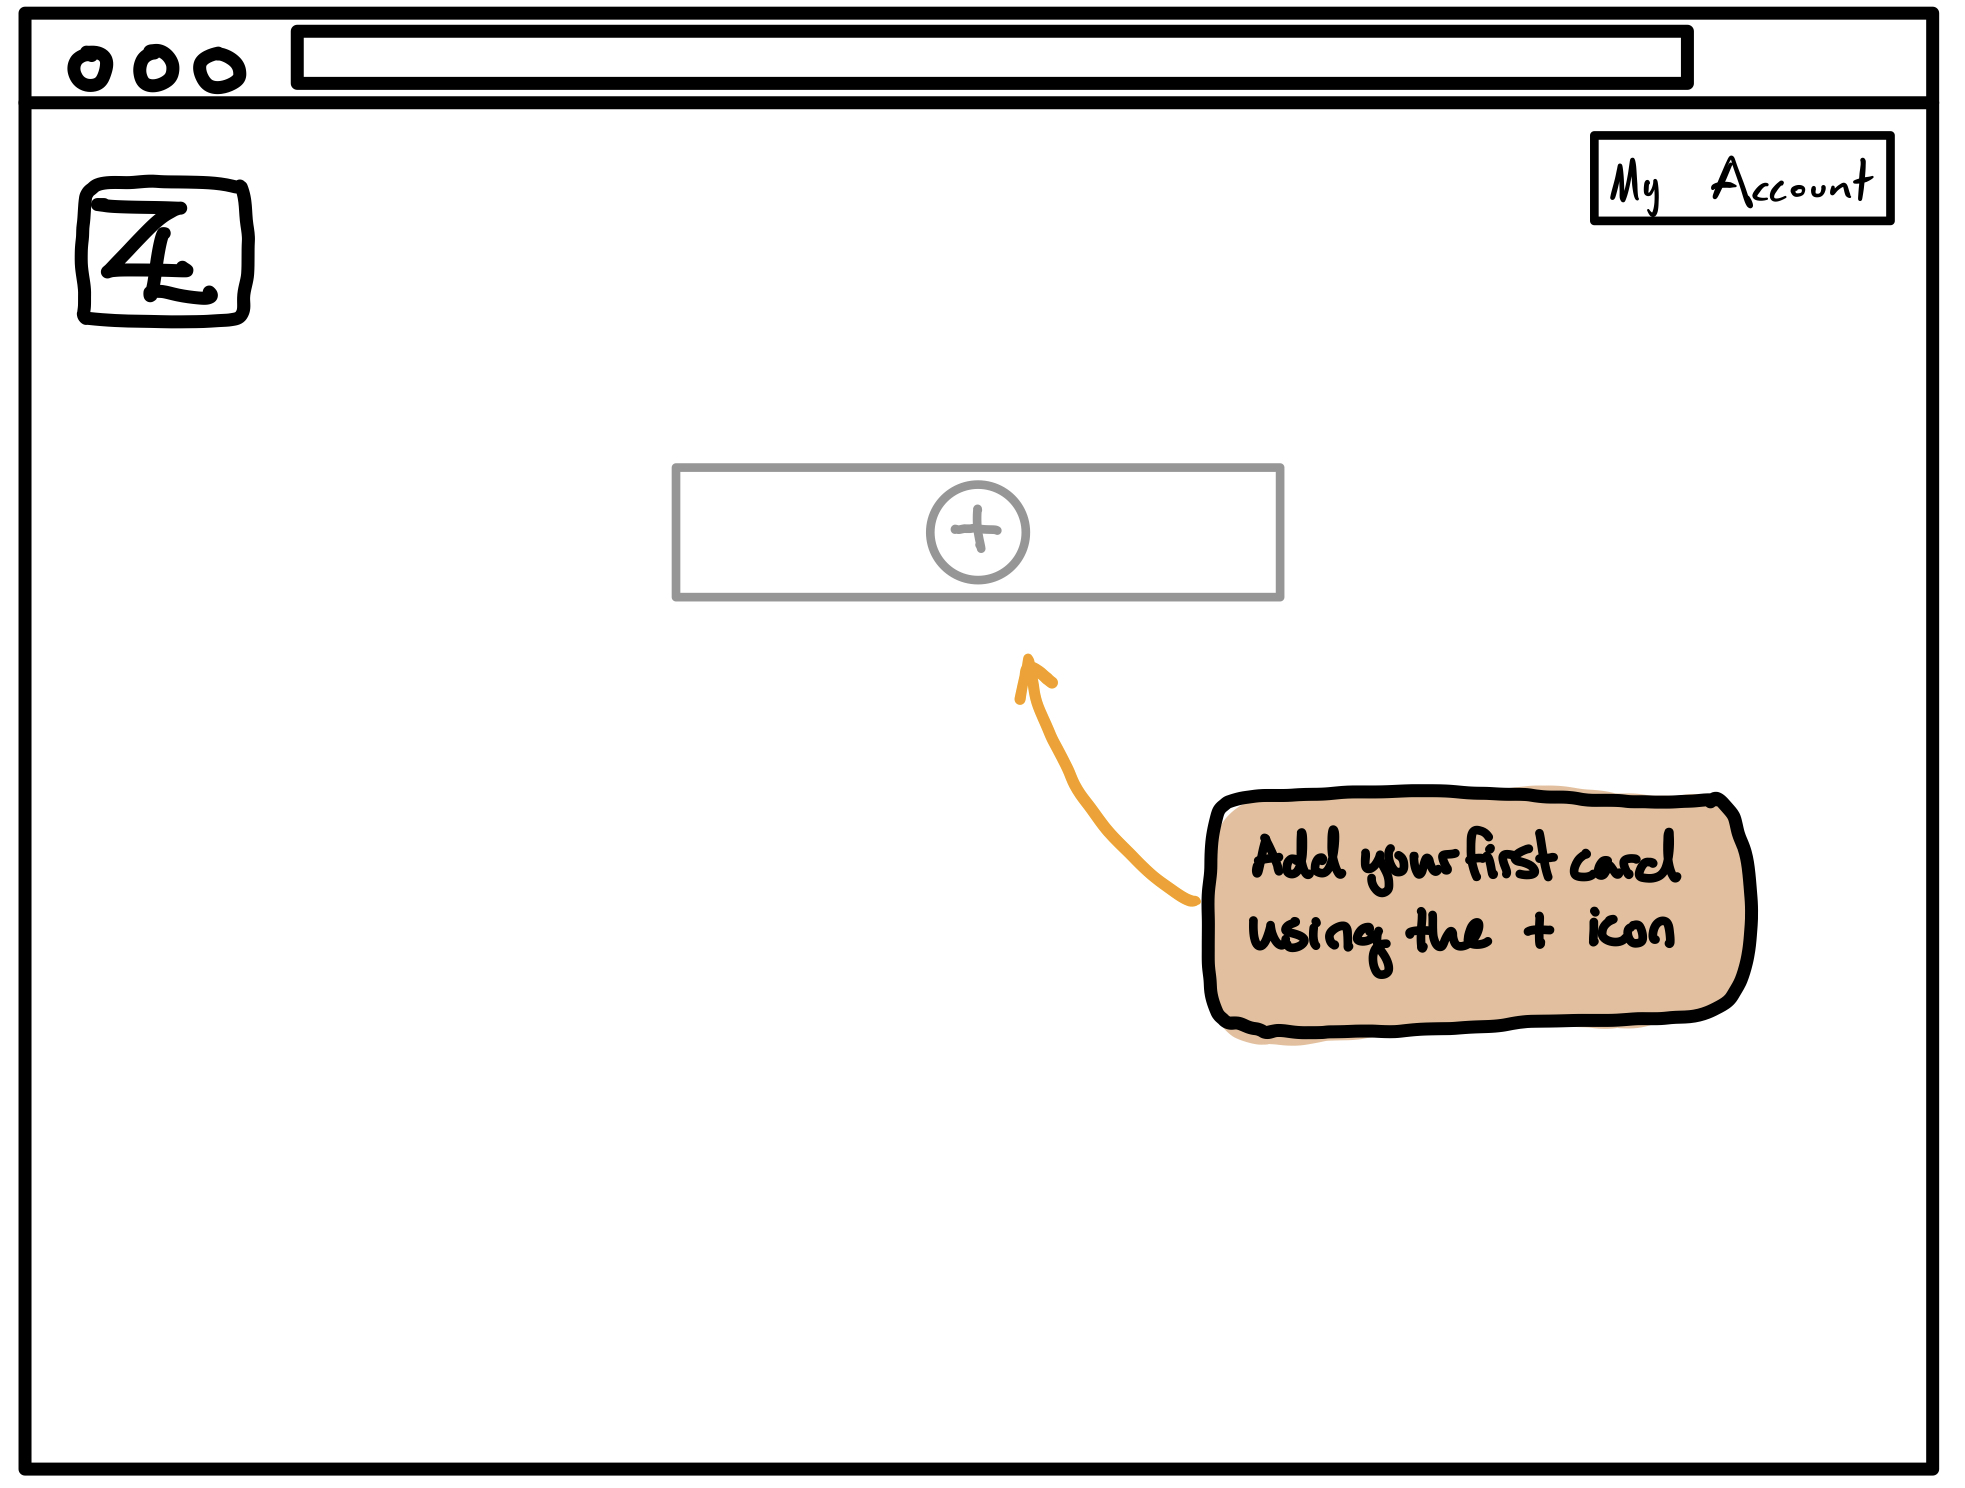
\includegraphics[width=0.98\paperwidth]{storyboard_images/card_list_page_newAcct.jpeg}}
    {\it After successfully creating an account or logging in, the user will be navigated to the Card List Page. A new account will have no cards, so only the "Add Card" button will appear on the Card List Page.}

    \clearpage
    {\bf \Large Create/Edit Card Page}
    \makebox[\textwidth]{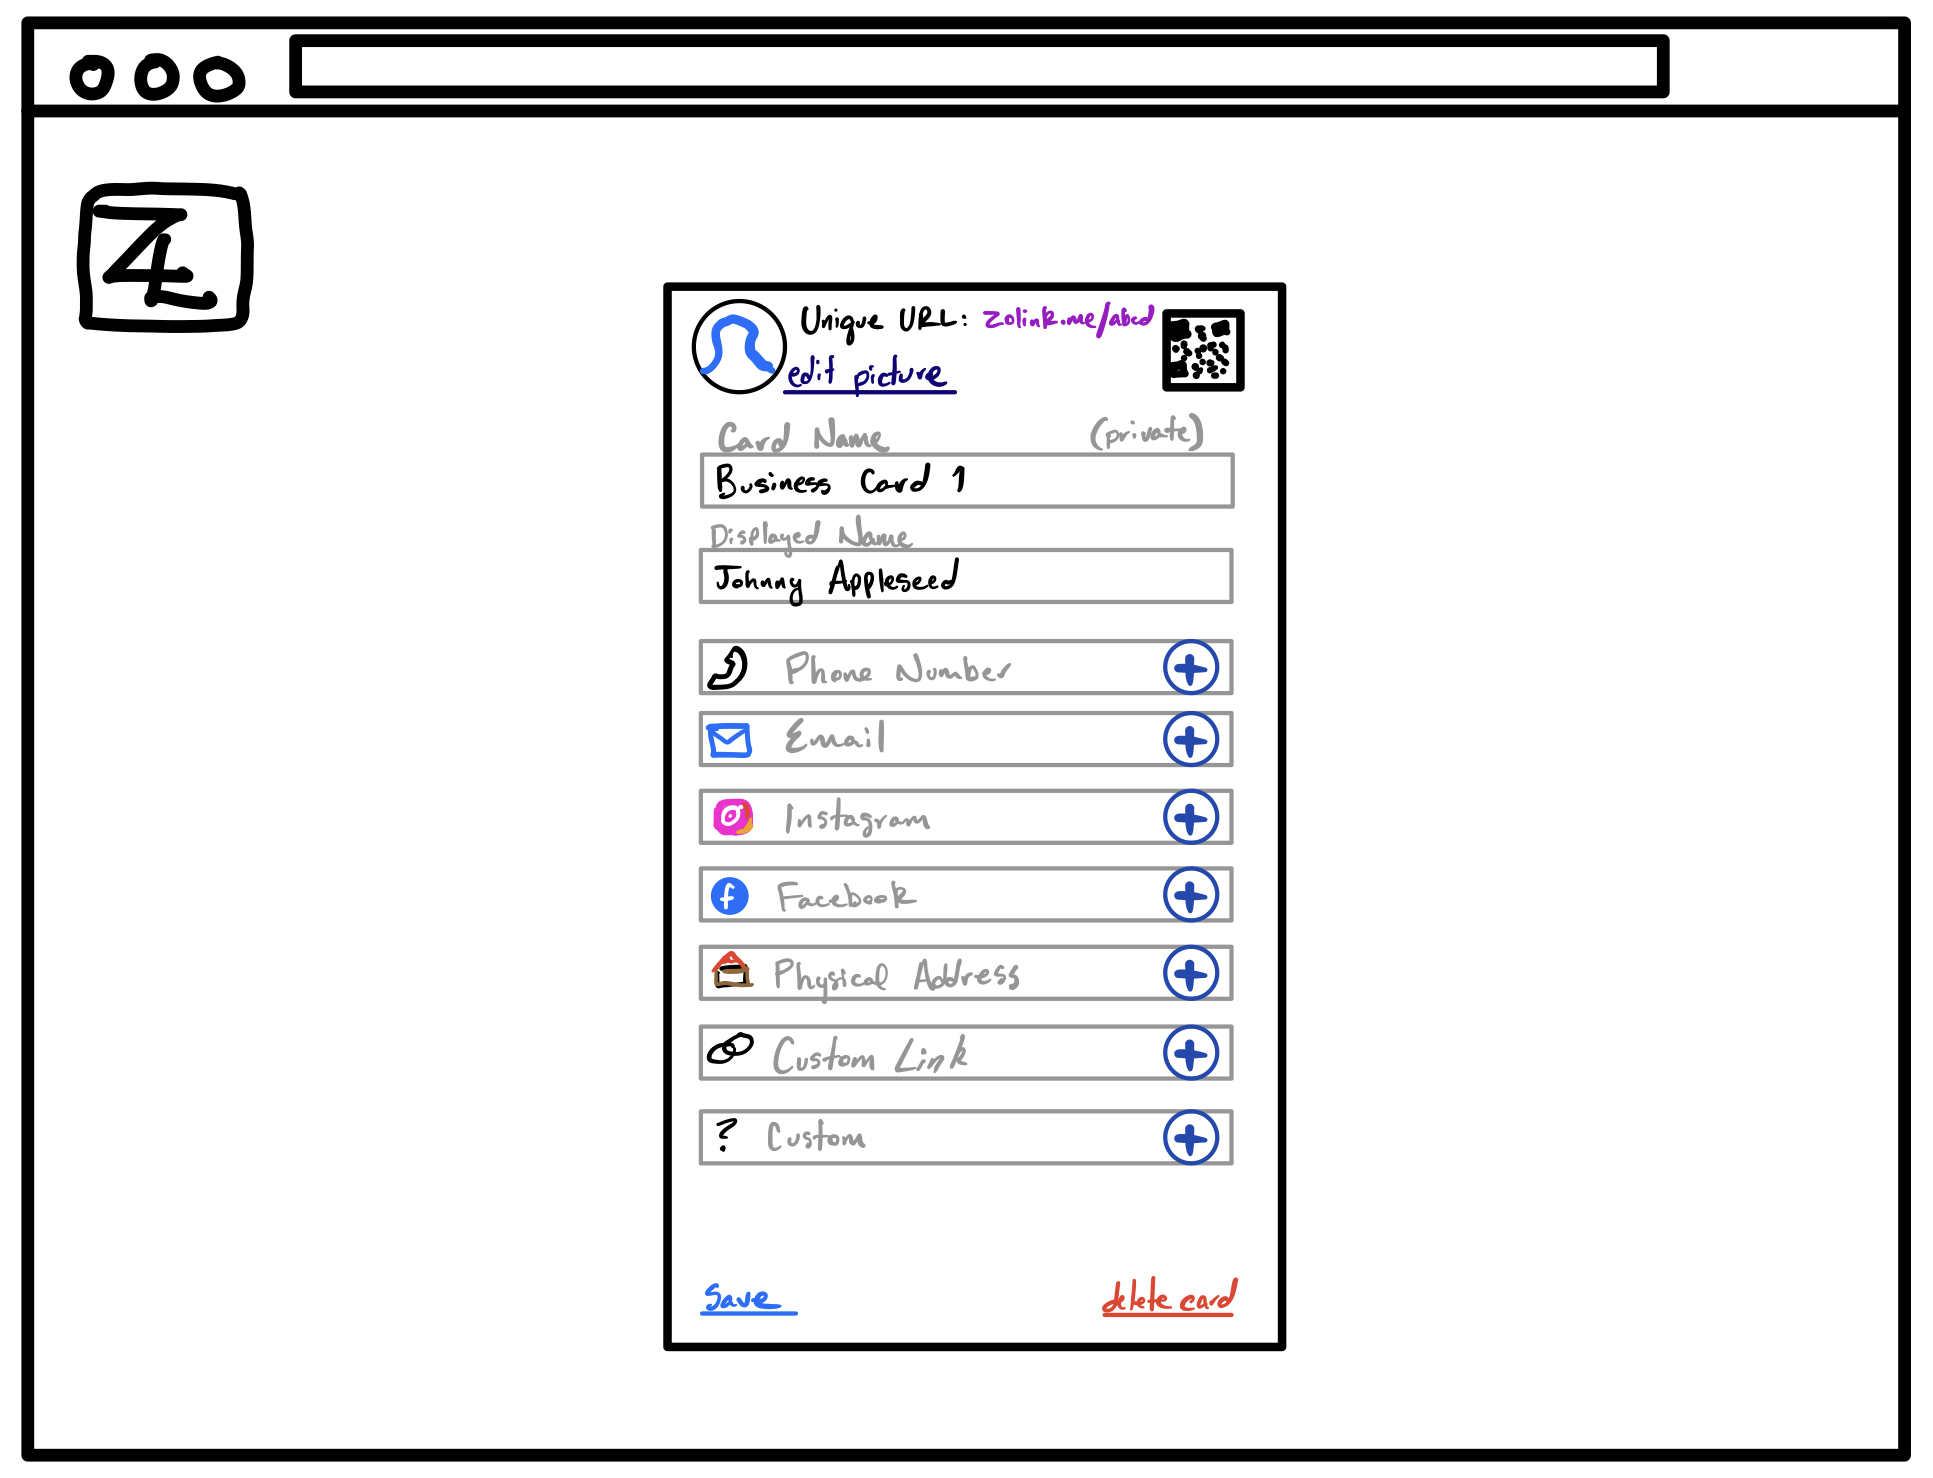
\includegraphics[width=0.98\paperwidth]{storyboard_images/create_edit_card.jpeg}}
    {\it The user can add their information to a card using this page. Attributes may be added or removed as needed.}

    \clearpage
    {\bf \Large Create/Edit Card Page (2)}
    \makebox[\textwidth]{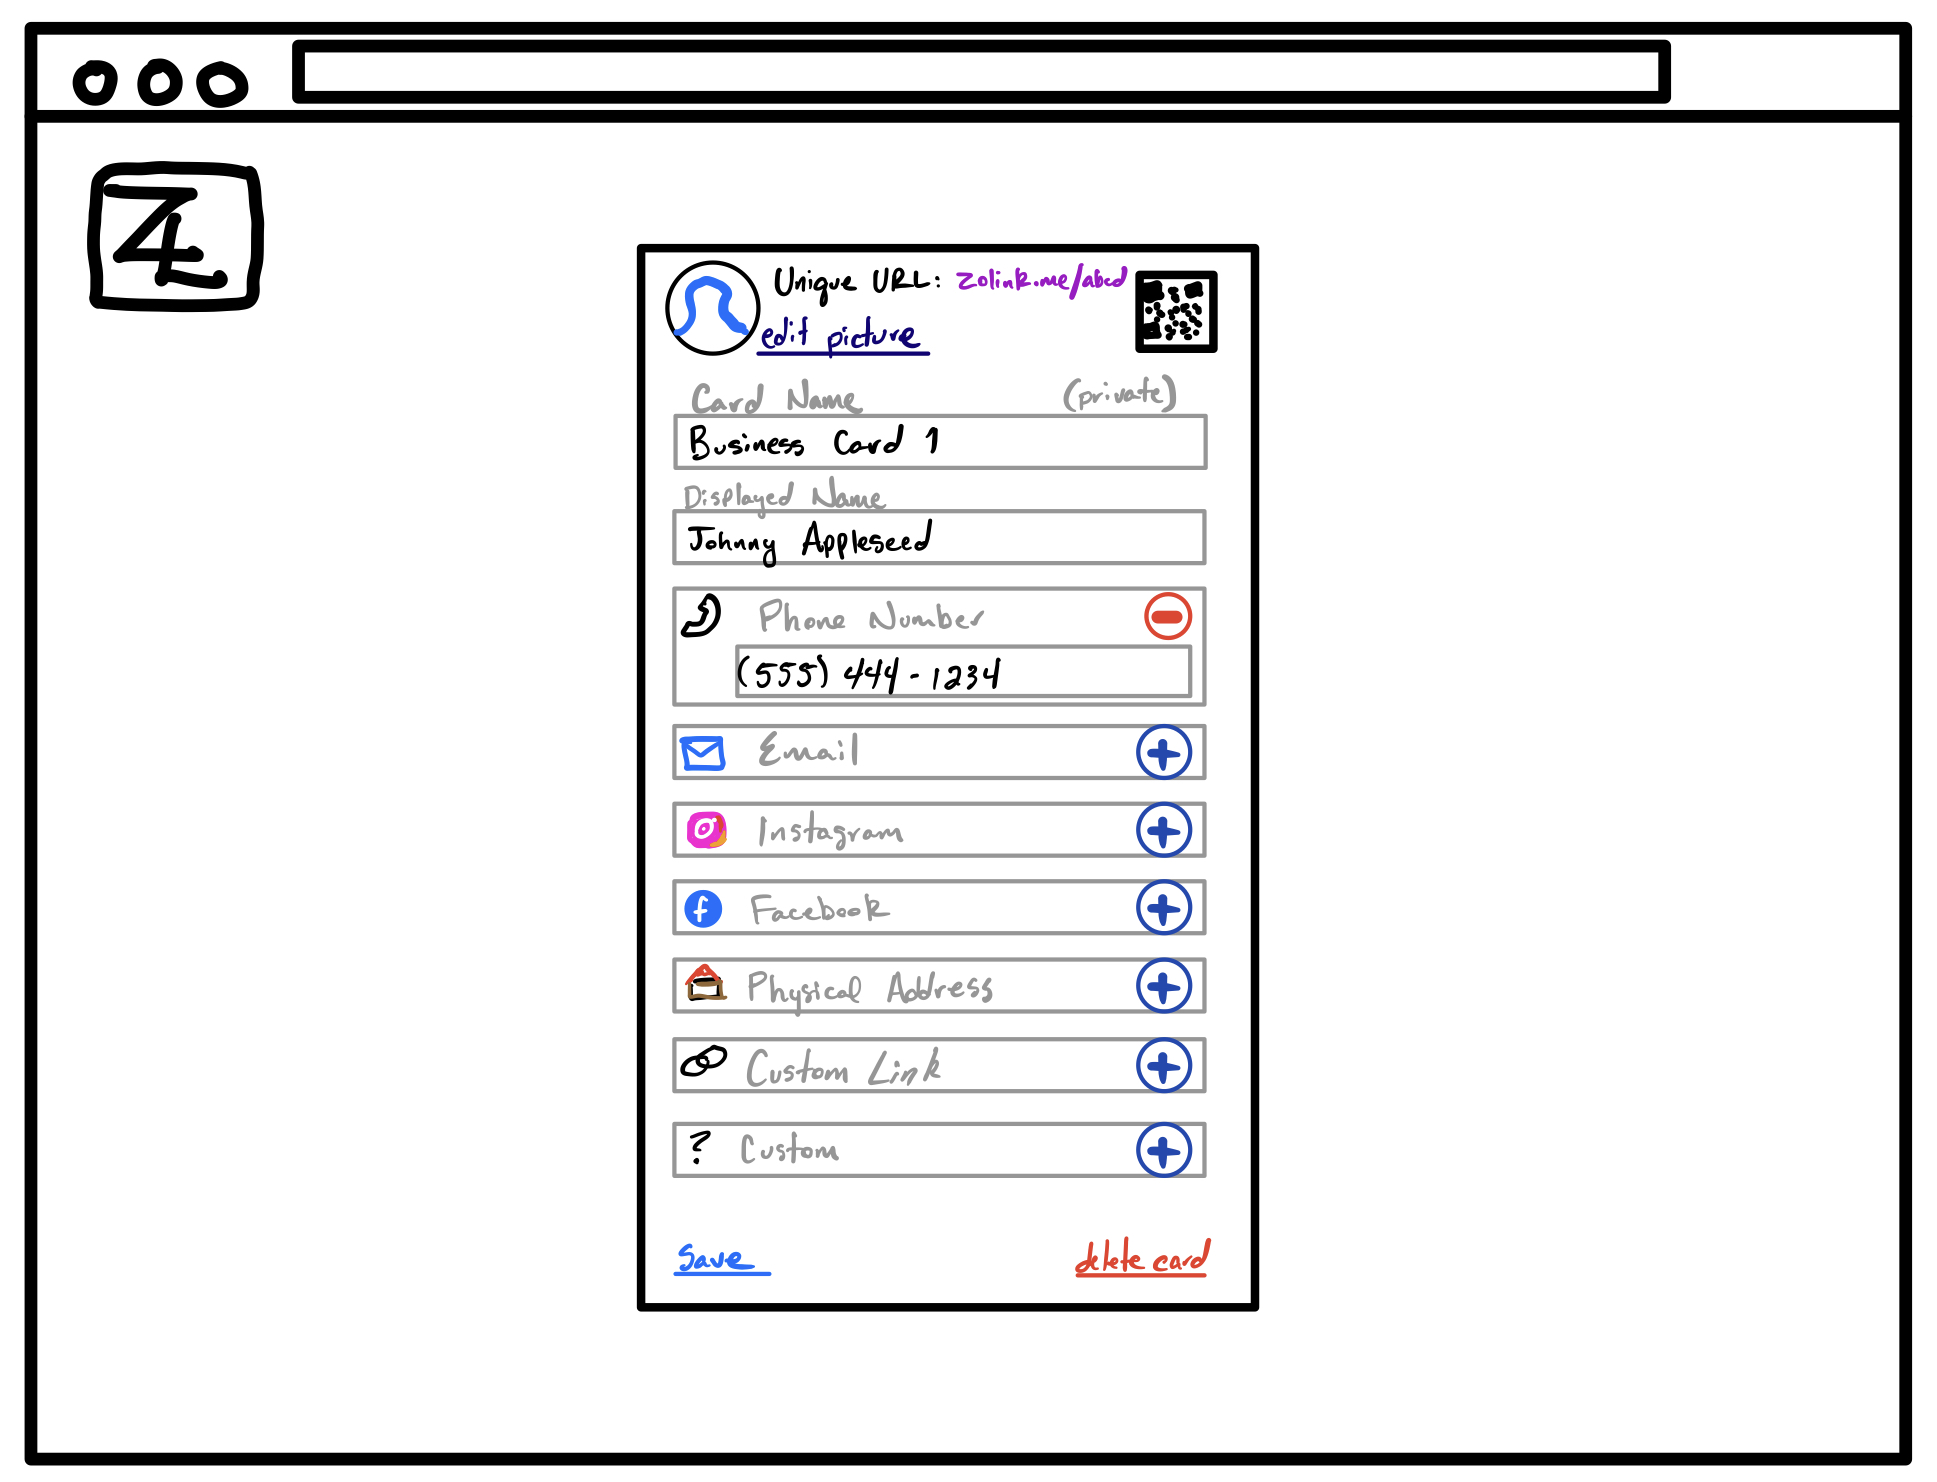
\includegraphics[width=0.98\paperwidth]{storyboard_images/create_edit_alt.jpeg}}
    {\it This sketch shows how the user will add their phone number.}

    \clearpage
    {\bf \Large Login Page}
    \makebox[\textwidth]{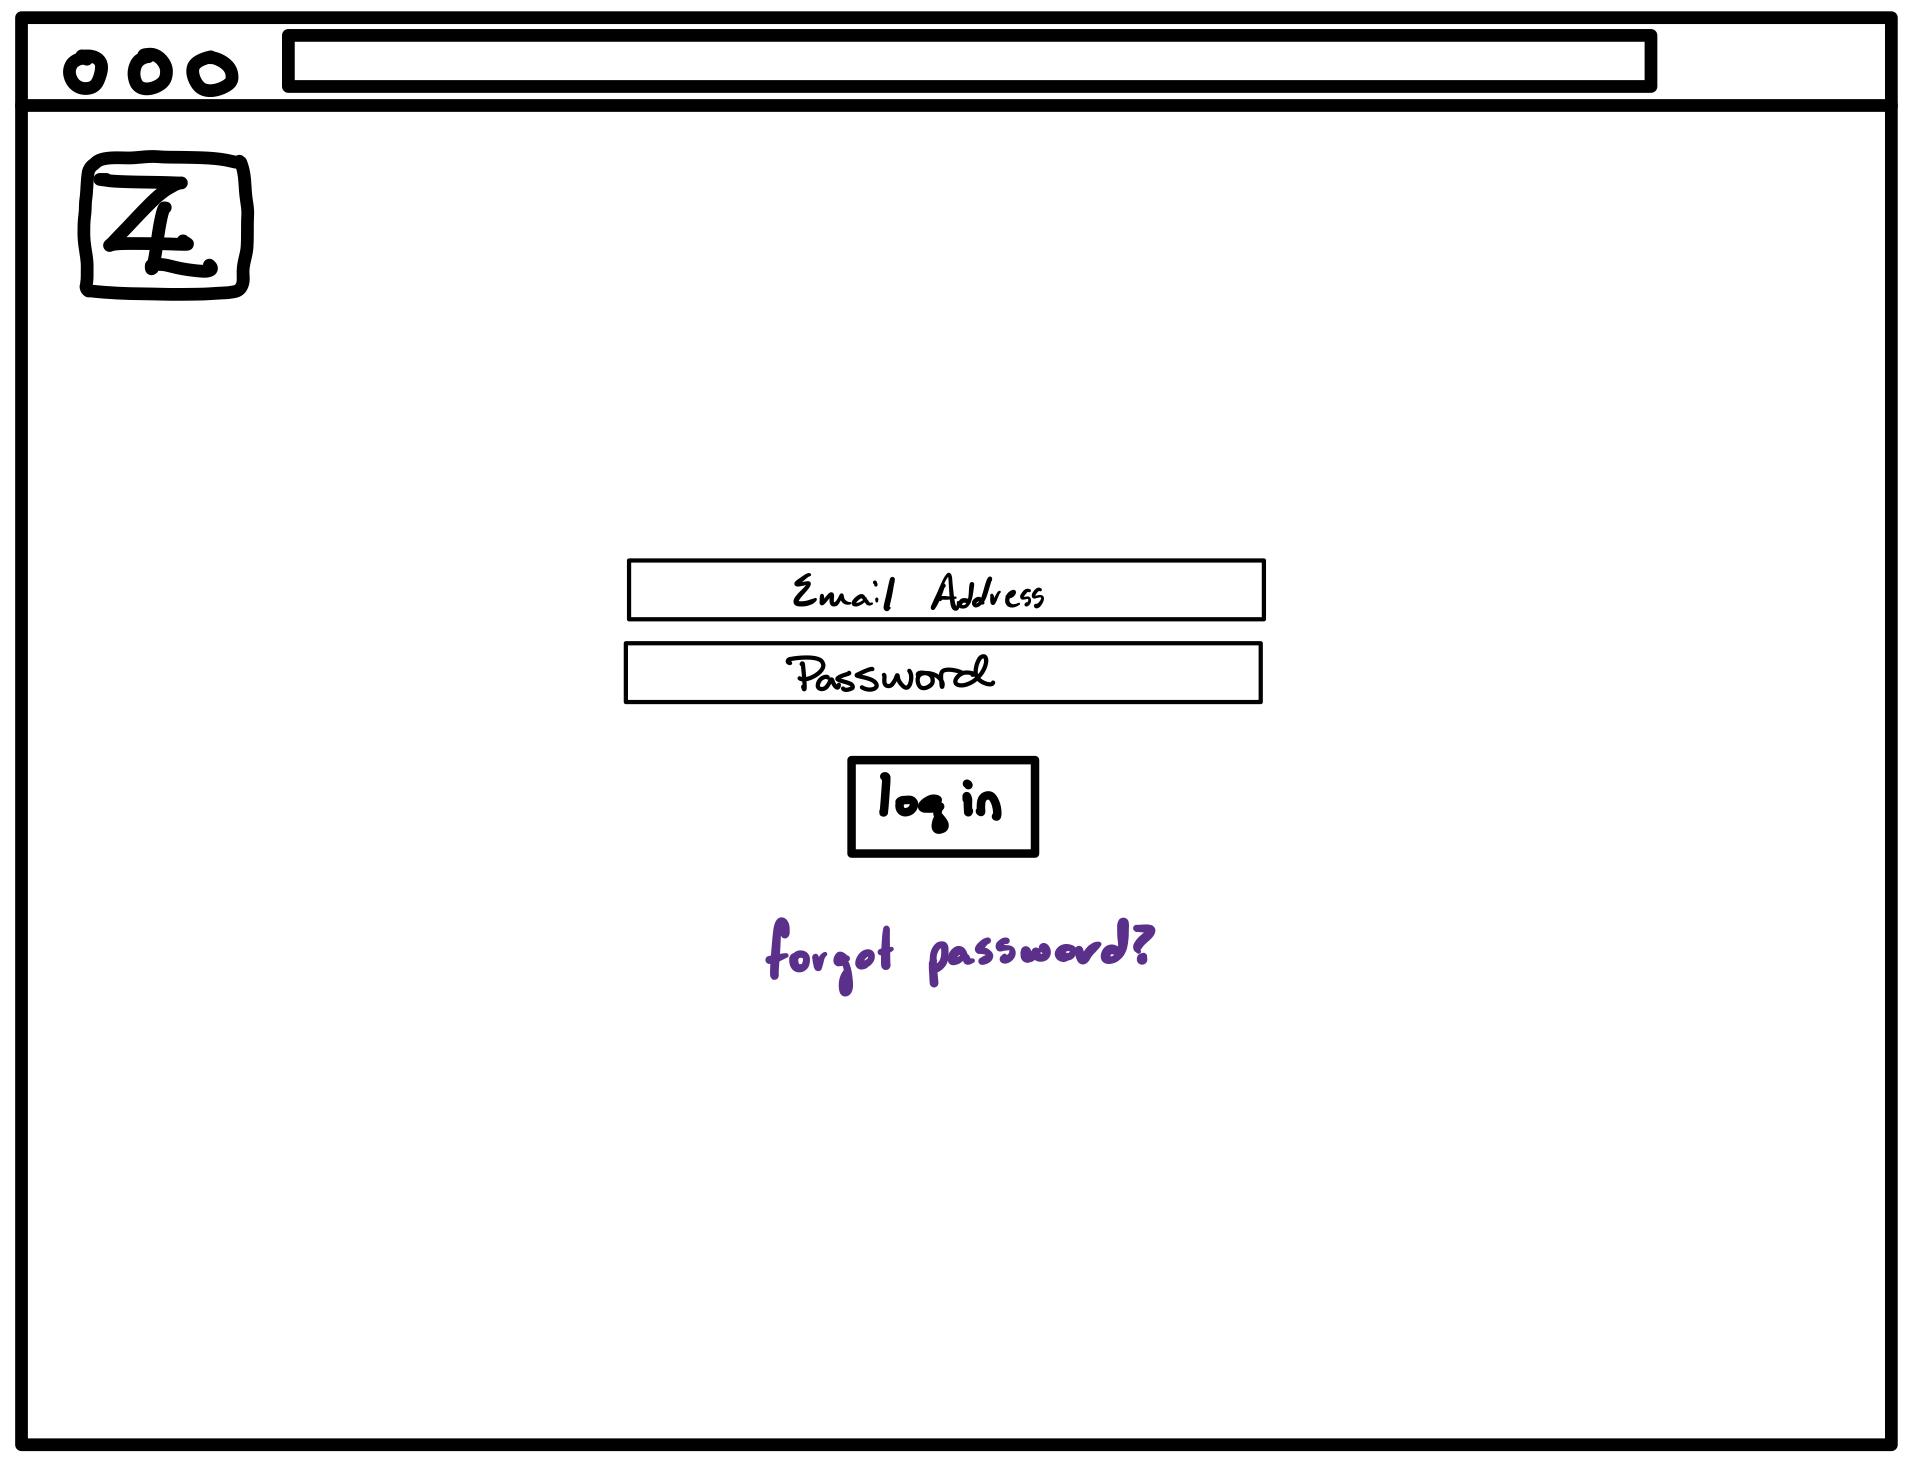
\includegraphics[width=0.98\paperwidth]{storyboard_images/login_page.jpeg}}

    \clearpage
    {\bf \Large Card List Page}
    \makebox[\textwidth]{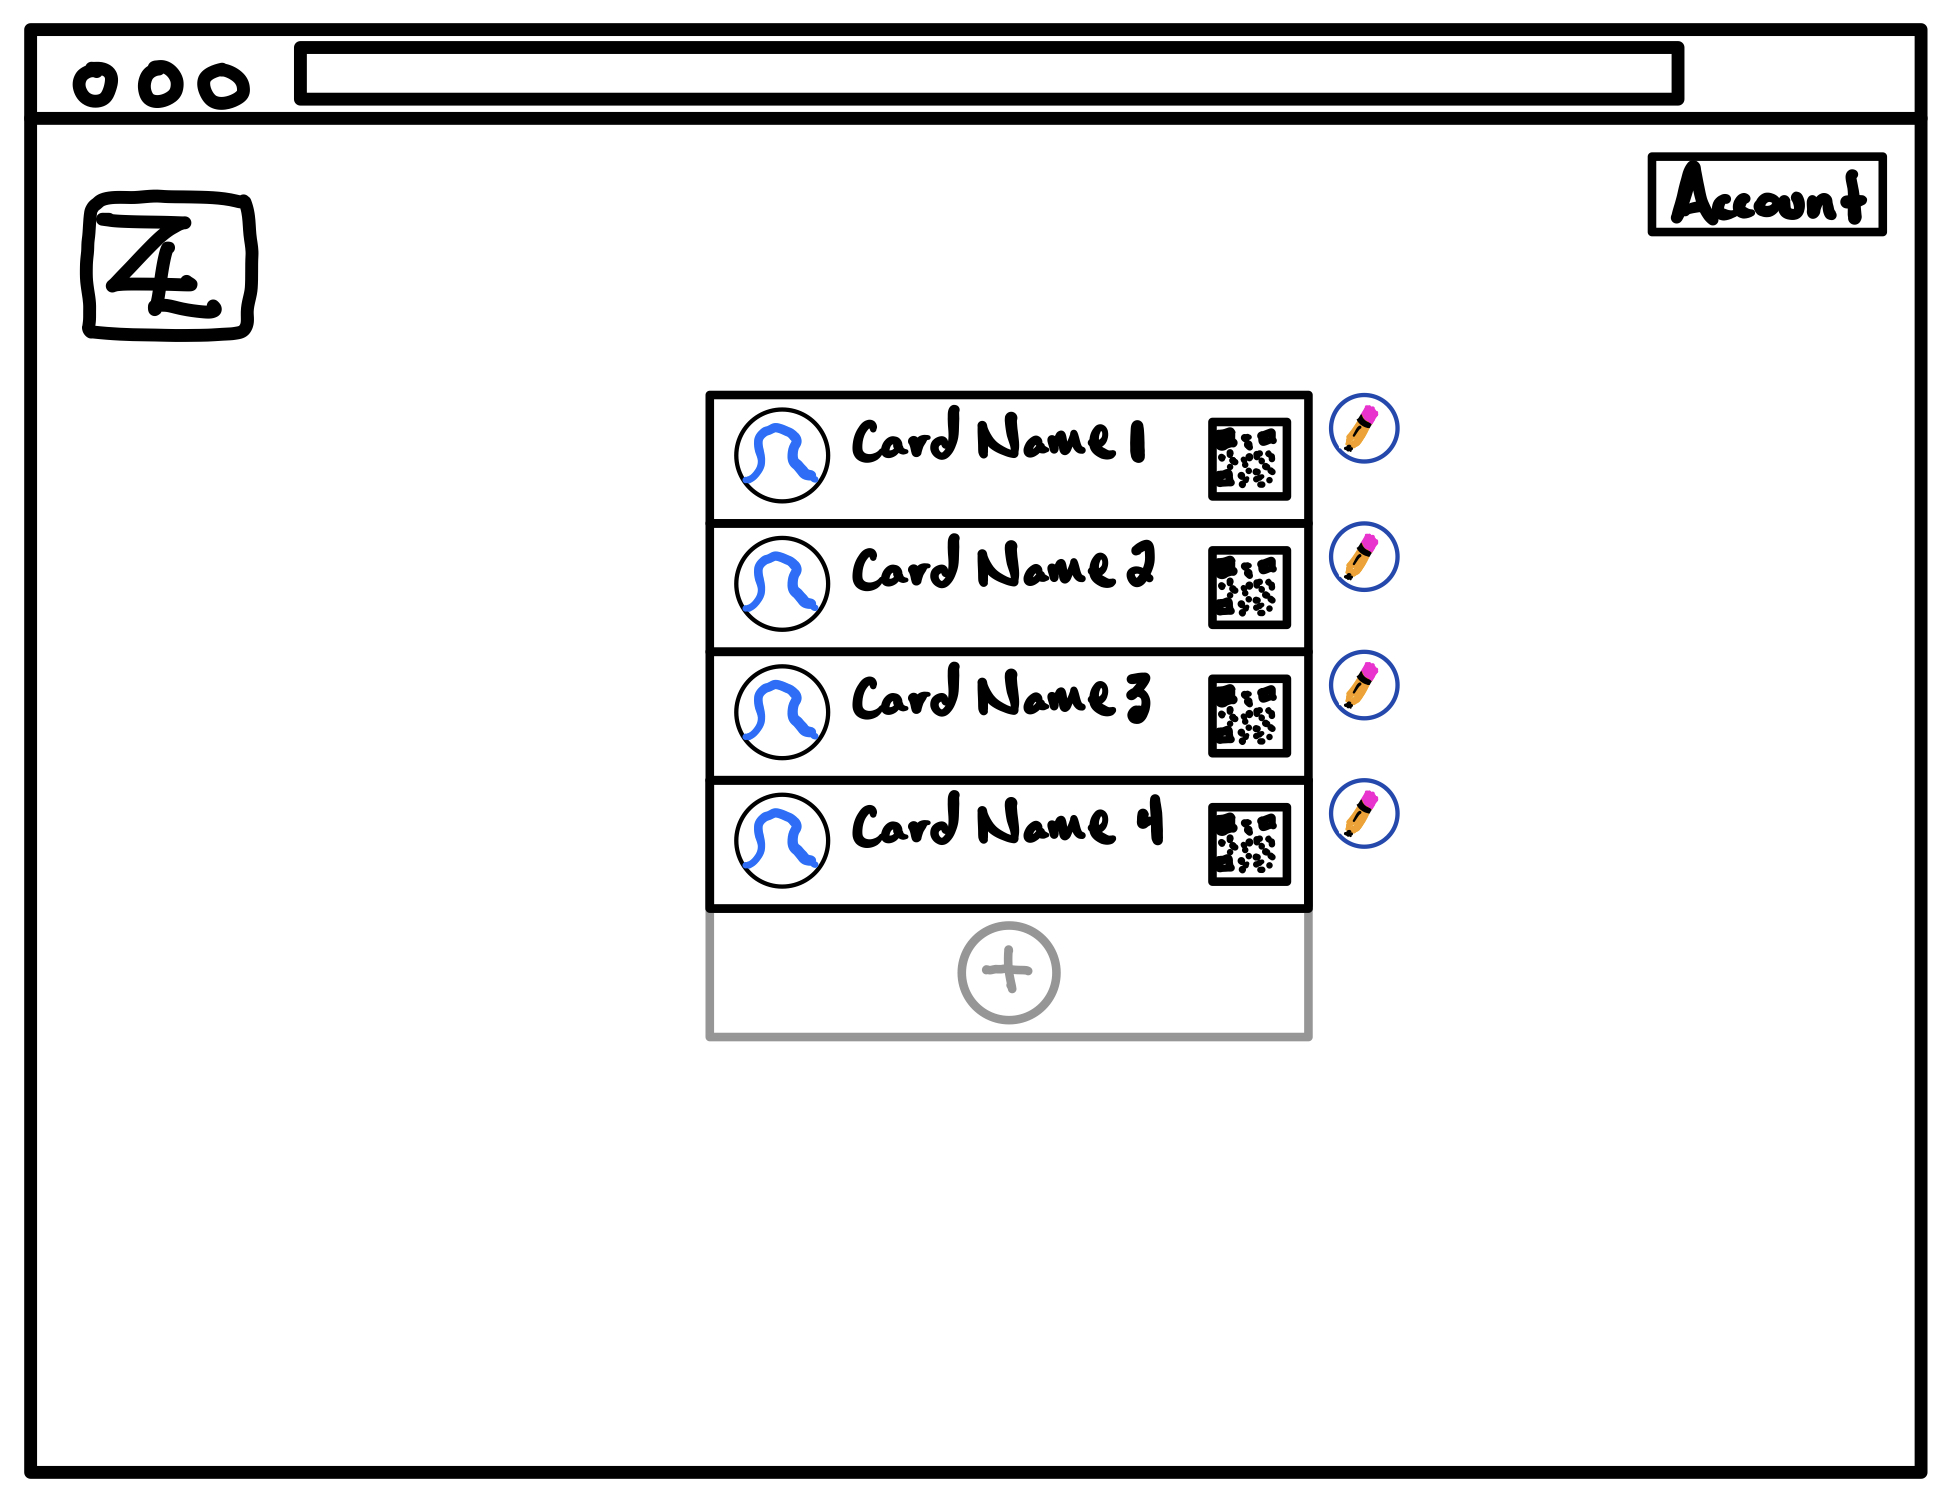
\includegraphics[width=0.98\paperwidth]{storyboard_images/card_list_page.jpeg}}
    {\it This is how the Card List Page will look after the user creates a few cards.}

    \clearpage
    {\bf \Large Card View Page}
    \makebox[\textwidth]{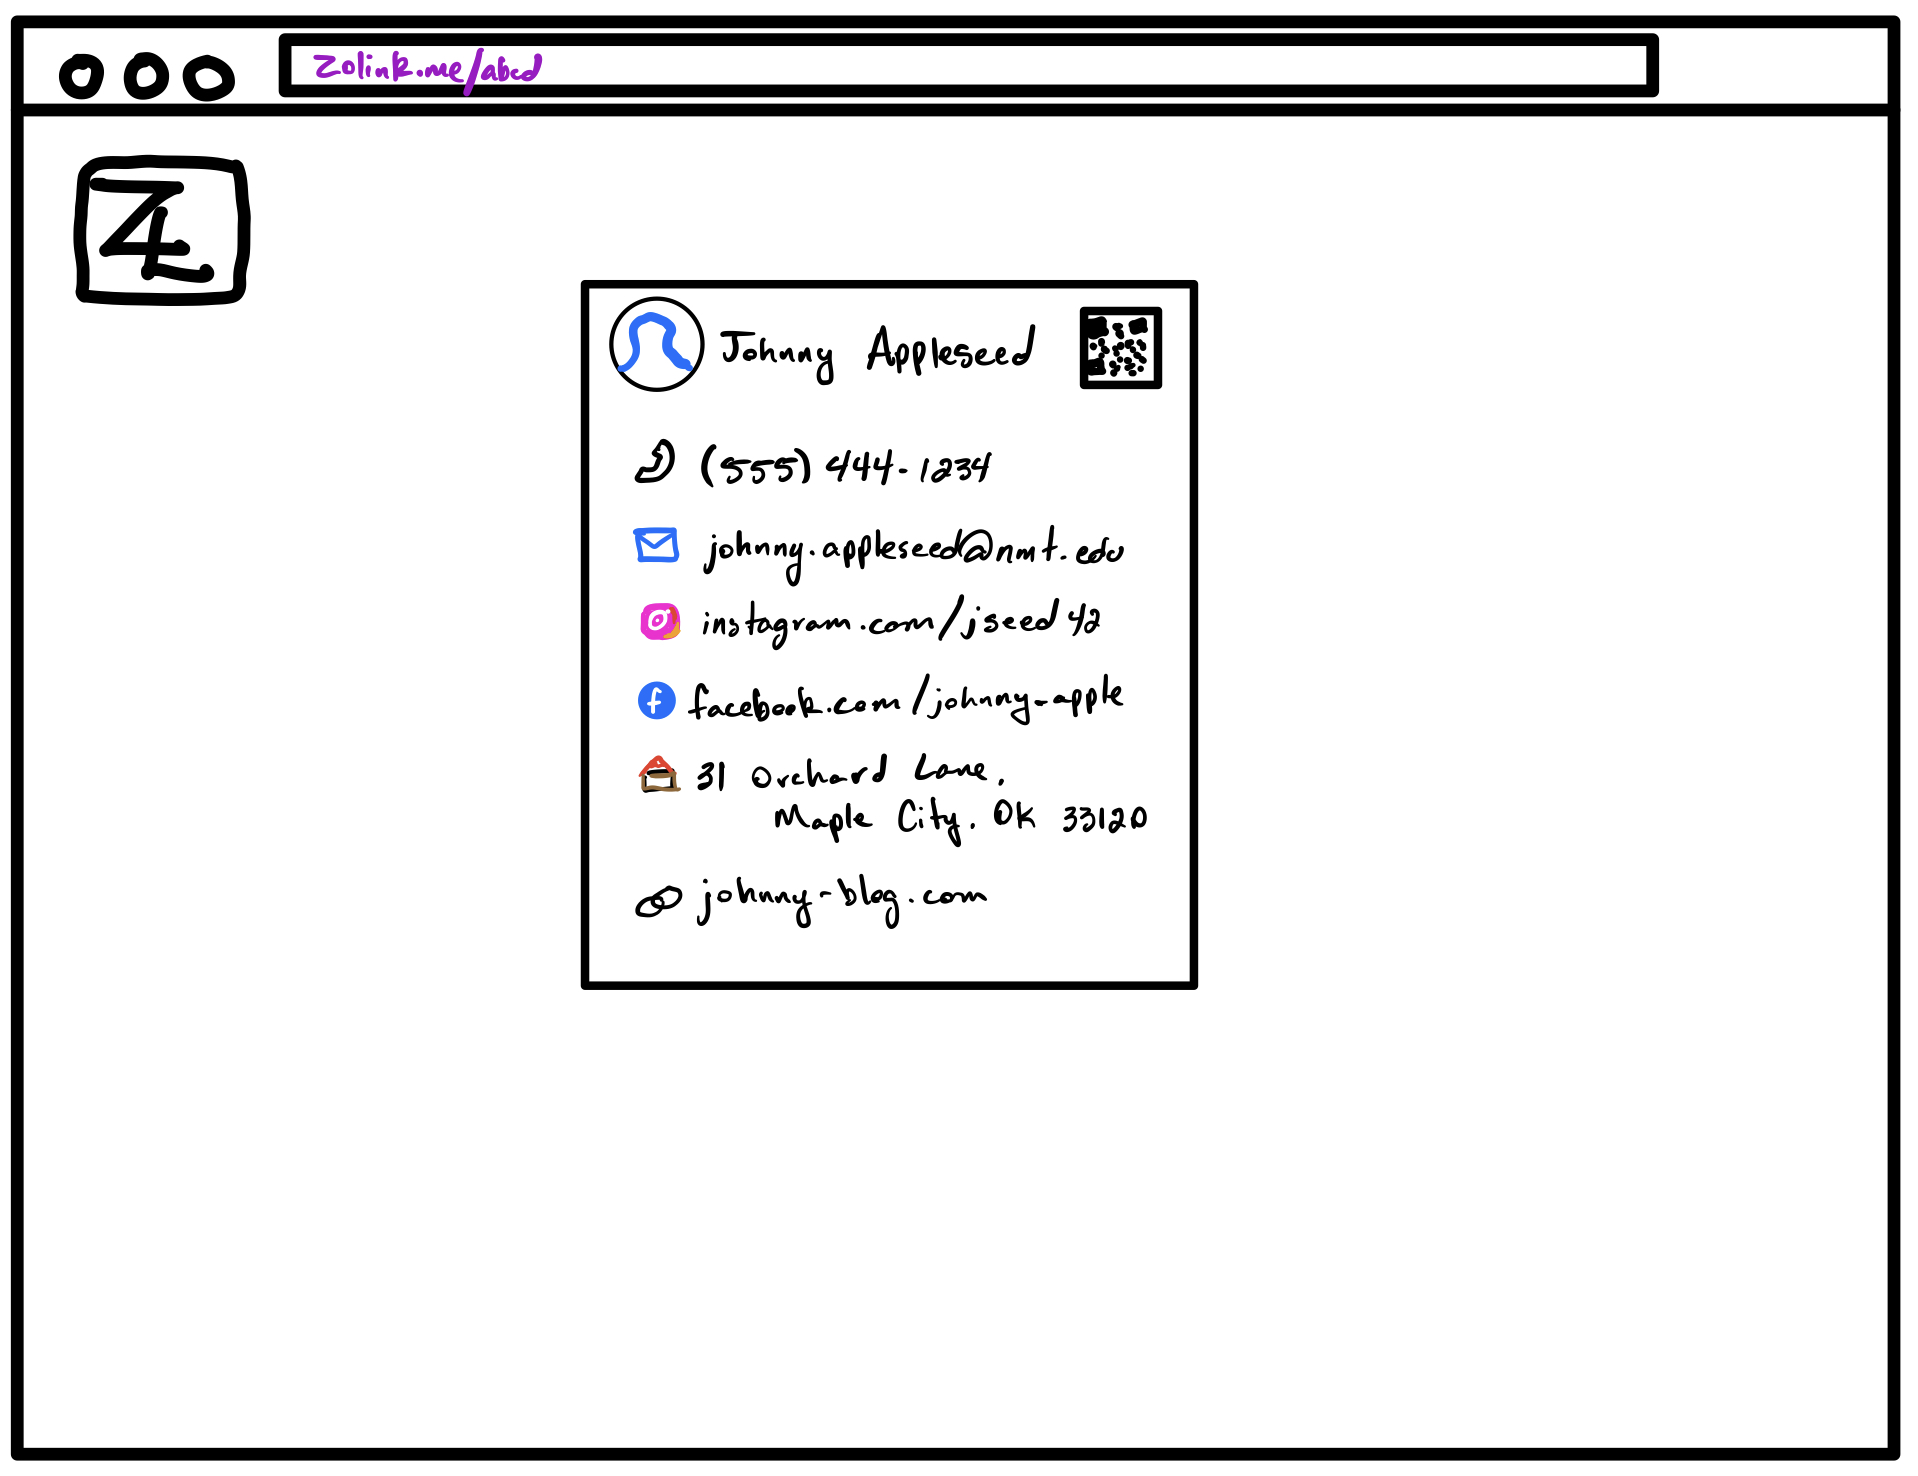
\includegraphics[width=0.98\paperwidth]{storyboard_images/card_page.jpeg}}
    {\it By clicking on one of the cards, the user may view it on this page.}

    \clearpage
    {\bf \Large Card QR Code View Page}
    \makebox[\textwidth]{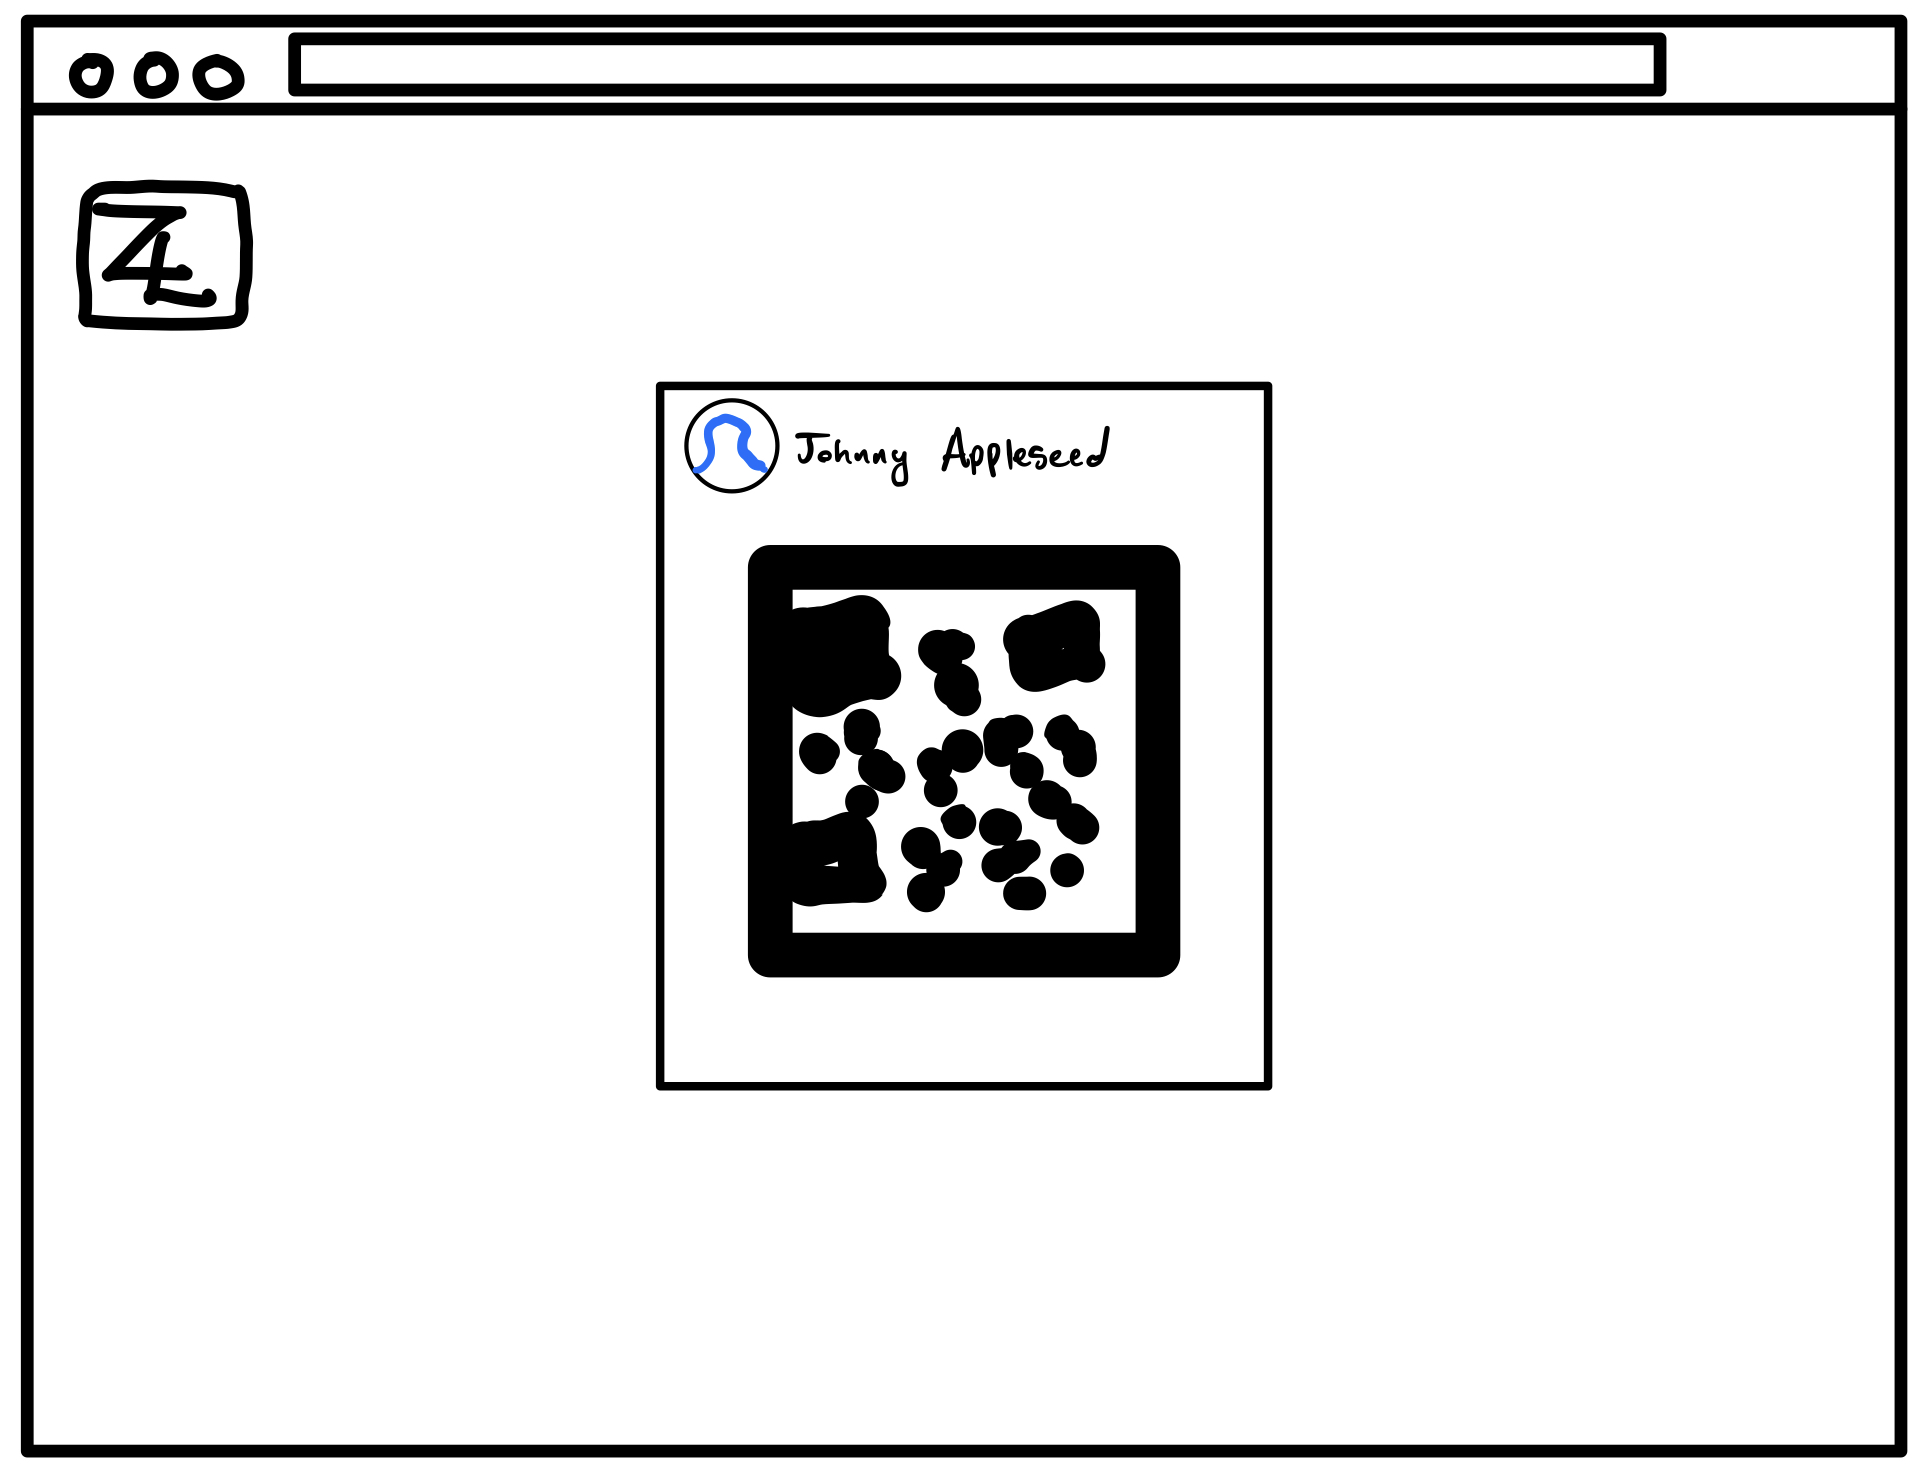
\includegraphics[width=0.98\paperwidth]{storyboard_images/qr_code_page.jpeg}}
    {\it By clicking the QR code on the Card View Page, the user may view the unique QR code for that card.}

    \clearpage
    {\bf \Large Account Page}
    \makebox[\textwidth]{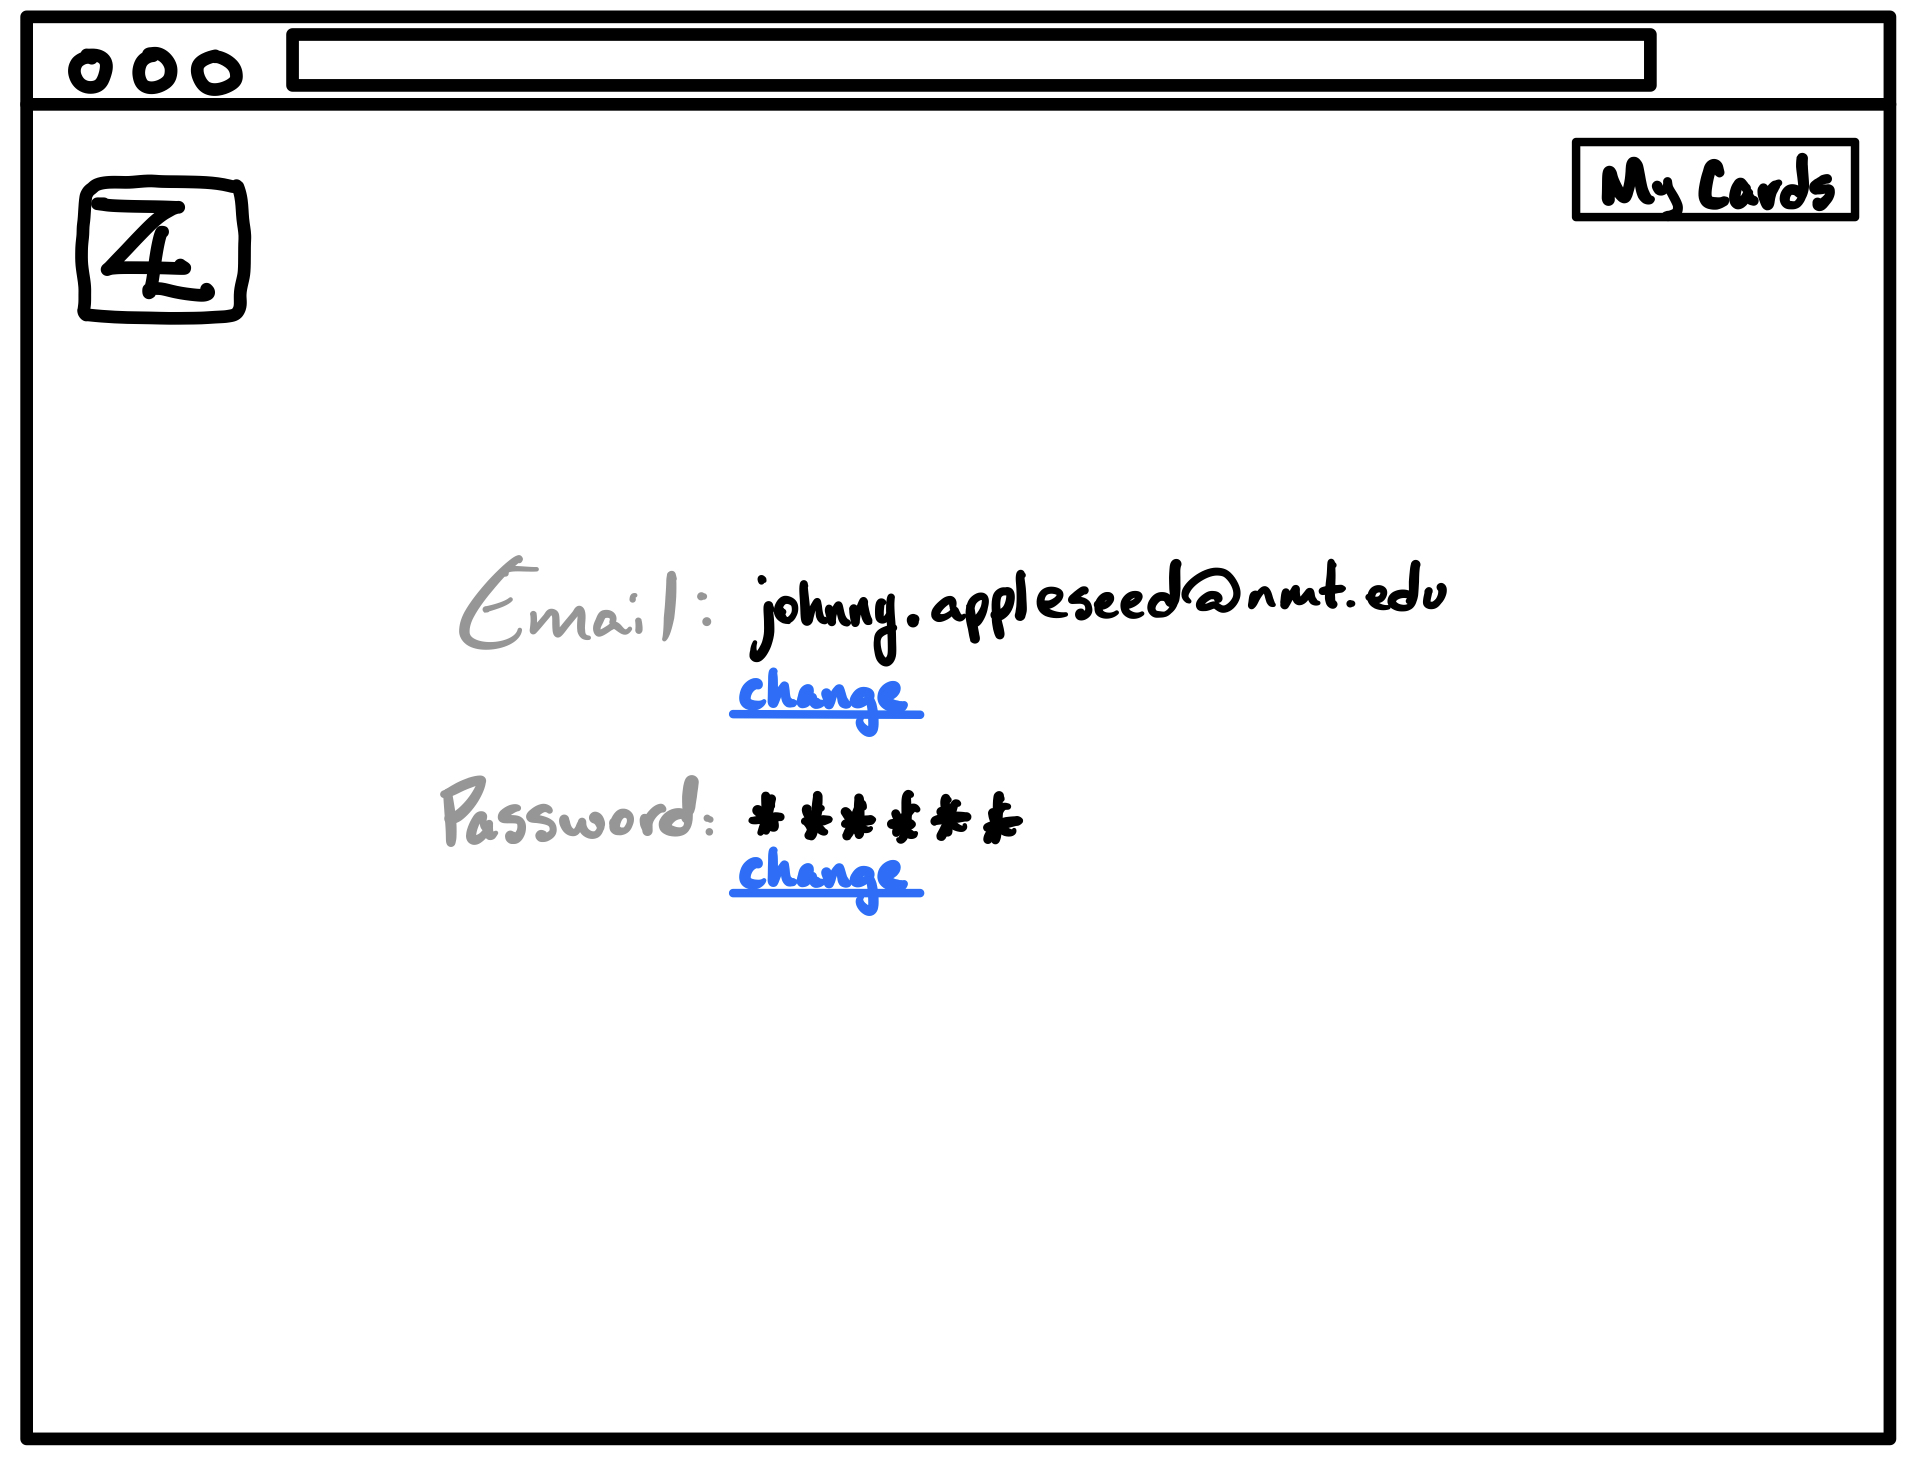
\includegraphics[width=0.98\paperwidth]{storyboard_images/account_page.jpeg}}
    {\it The user may change their email and password on this page.}

\end{center}

\clearpage
\section{ER Diagram}

\begin{enumerate}[4.a.]
    \item ER Diagram\\
    The purpose of this section is to represent how our database will work for our website. We have presented this through 
    an ER Diagram that acts as a blueprint for how we will setup our database. The Diagram shows the relationships between 
    different types of data as well as underlying important information such as primary keys. The ER Diagram is shown below as well 
    as an in-depth description of our table design. 
    
     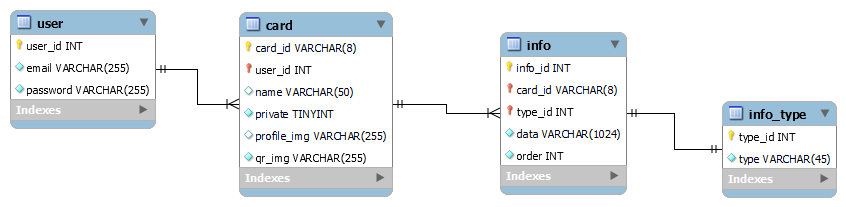
\includegraphics[width=\linewidth]{er.png}
    \item Table Design.\\
    User Table
        \begin{itemize}
            \item The user table is for all the data necessary to identify each user.
            \item The primary key, user\_id, is a unique integer value auto-incremented for each new user.
            \item The email field has the type VARCHAR(255) and stores the user’s unique email used to log on.
            \item The password field has the type VARCHAR(255) and stores the user’s password used to log on (hashed).
        \end{itemize}
    Card Table
            \begin{itemize}
            \item The Card table has a one-to-many relationship with the user table and contains fields necessary for the card’s attributes.
            \item The primary key, card\_id, is a unique integer value auto-incremented for each new card.
            \item The foreign key, user\_id, relates the card to the unique user in the user table and is of type INT.
            \item The name field has the type VARCHAR(50) and stores the user-entered name for the given card.
            \item The private field has type tinyint and stores 0 (card is public) or 1 (card is private).
            \item The profile\_img field has the type VARCHAR(255) and stores the path to the user-uploaded profile image.
            \item The qr\_img field has the type VARCHAR(255) and stores the path to the unique QR code image.
        \end{itemize}
    Info Table
            \begin{itemize}
            \item This table stores the information in each card (social media accounts, emails, etc.).
            \item The info table has a one-to-many relationship with the card table and a one-to-one relationship with the info type table.
            \item The primary key, info\_id, is a unique INT (automatically incremented each new info entry)
            \item The foreign key, card\_id, relates the information to the given card.
            \item The foreign key, type\_id, assigns the information type specified in the info\_type table.
            \item The data field has the type VARCHAR(1024) and stores the user-entered info data.
            \item The order field stores an INT value representing the user-chosen ordering of the card info.
        \end{itemize}
    Info\_type Table
            \begin{itemize}
            \item This table stores the different types of information included on a card.
            \item The type\_id field is an automatically incremented and unique INT value.
            \item The type field stores the unique name of the information type (“email,” “phone,” etc.) in a VARCHAR(45).
        \end{itemize}
    \footnotesize
    \singlespacing
    \begin{tabular}{|c|c|c|c|c|c|c|c|}
        \hline
        \multicolumn{8}{|l|}{\bf user}\\
        \hline
        \hline
        \thead{Primary\\Key} & \thead{Field\\Name} & \thead{Data\\Type} & \thead{Not\\Null} & Unique & Binary & \thead{Foreign\\Key} & Comments \\
        \hline
        \checkmark & user\_id & int & \checkmark & \checkmark & & & \makecell{Automatically incremented\\for each new user.}\\
        \hline
         & email & varchar(255) & \checkmark & \checkmark & & & \makecell{Used to log on.}\\
        \hline
        & password & varchar(255) & \checkmark & & & & \makecell{Used to log on, hashed.}\\
        \hline
    \end{tabular}
    
    \vspace{1cm}
    
    \begin{tabular}{|c|c|c|c|c|c|c|c|}
        \hline
        \multicolumn{8}{|l|}{{\bf card} \ntab\ntab {\it one-to-many relationship with user}}\\
        \hline
        \hline
        \thead{Primary\\Key} & \thead{Field\\Name} & \thead{Data\\Type} & \thead{Not\\Null} & Unique & Binary & \thead{Foreign\\Key} & Comments \\
        \hline
        \checkmark & card\_id & varchar(8) & \checkmark & \checkmark & & & \makecell{Automatically incremented\\for each new card.}\\
        \hline
         & user\_id & int & \checkmark & & & \checkmark & \makecell{Identify which user\\owns each card.}\\
        \hline
         & name & varchar(50) & & & & & \makecell{Allows the user\\to name each card.}\\
        \hline
         & private & tinyint & \checkmark & & & & \makecell{0 = public\\1 = private}\\
        \hline
        & profile\_img & varchar(255) & & & & & \makecell{Path to user-uploaded\\profile image.}\\
        \hline
        & qr\_img & varchar(255) & \checkmark & \checkmark & & & \makecell{Path to unique QR\\image linked to card.}\\
        \hline
    \end{tabular}
    
        \vspace{1cm}
    
    \begin{tabular}{|c|c|c|c|c|c|c|c|}
        \hline
        \multicolumn{8}{|l|}{{\bf info} \ntab\ntab {\it one-to-many relationship with card}}\\
        \multicolumn{8}{|l|}{\ntab\ntab\ntab {\it one-to-one relationship with info\_type}}\\
        \hline
        \hline
        \thead{Primary\\Key} & \thead{Field\\Name} & \thead{Data\\Type} & \thead{Not\\Null} & Unique & Binary & \thead{Foreign\\Key} & Comments \\
        \hline
        \checkmark & info\_id & int & \checkmark & \checkmark & & & \makecell{Automatically incremented\\for each new info entry.}\\
        \hline
         & card\_id & varchar(8) & \checkmark & & & \checkmark & \makecell{Identify which card\\each entry goes with.}\\
        \hline
         & type\_id & int & \checkmark & & & \checkmark & \makecell{Assigns info type\\from info\_type table.}\\
        \hline
        & data & varchar(1024) & \checkmark & & & & \makecell{User-entered info data.}\\
        \hline
        & order & int & \checkmark & & & & \makecell{Allow user to choose\\ordering of card info.}\\
        \hline
    \end{tabular}
    
    \vspace{1cm}
    
    \begin{tabular}{|c|c|c|c|c|c|c|c|}
        \hline
        \multicolumn{8}{|l|}{{\bf info\_type}}\\
        \hline
        \hline
        \thead{Primary\\Key} & \thead{Field\\Name} & \thead{Data\\Type} & \thead{Not\\Null} & Unique & Binary & \thead{Foreign\\Key} & Comments \\
        \hline
        \checkmark & type\_id & int & \checkmark & \checkmark & & & \makecell{Automatically incremented\\for each new info type.}\\
        \hline
         & type & varchar(45) & \checkmark & \checkmark & & & \makecell{Name of the info type\\e.g. "email", "phone".}\\
        \hline
    \end{tabular}
    
    
    
\end{enumerate}

\clearpage
\section{System Architecture}
\begin{enumerate}[5.a.]
	\item MVC: 
	
	
		
	\makebox[\textwidth]{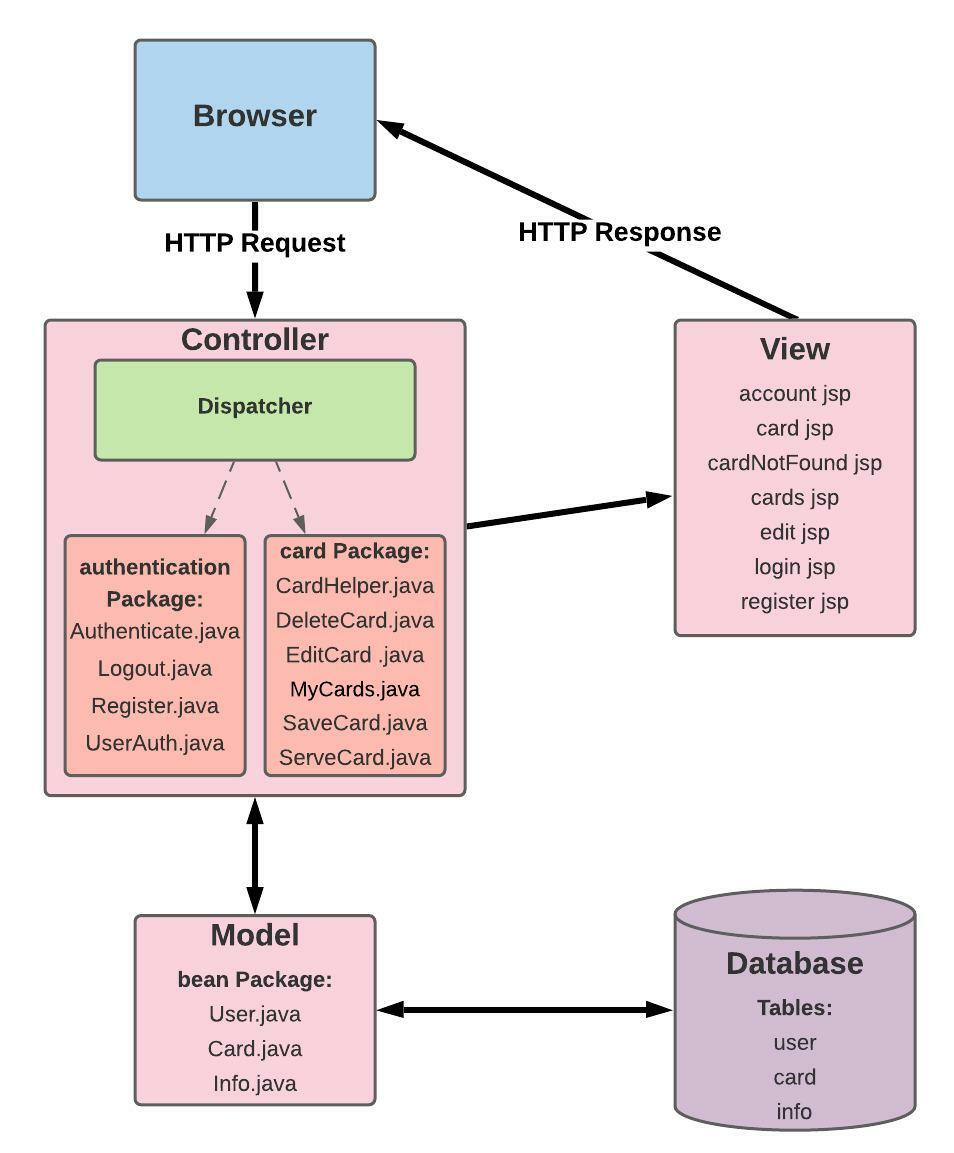
\includegraphics[width=0.55\paperwidth]{mvc.jpeg}}
	
	
	\makebox[\textwidth]{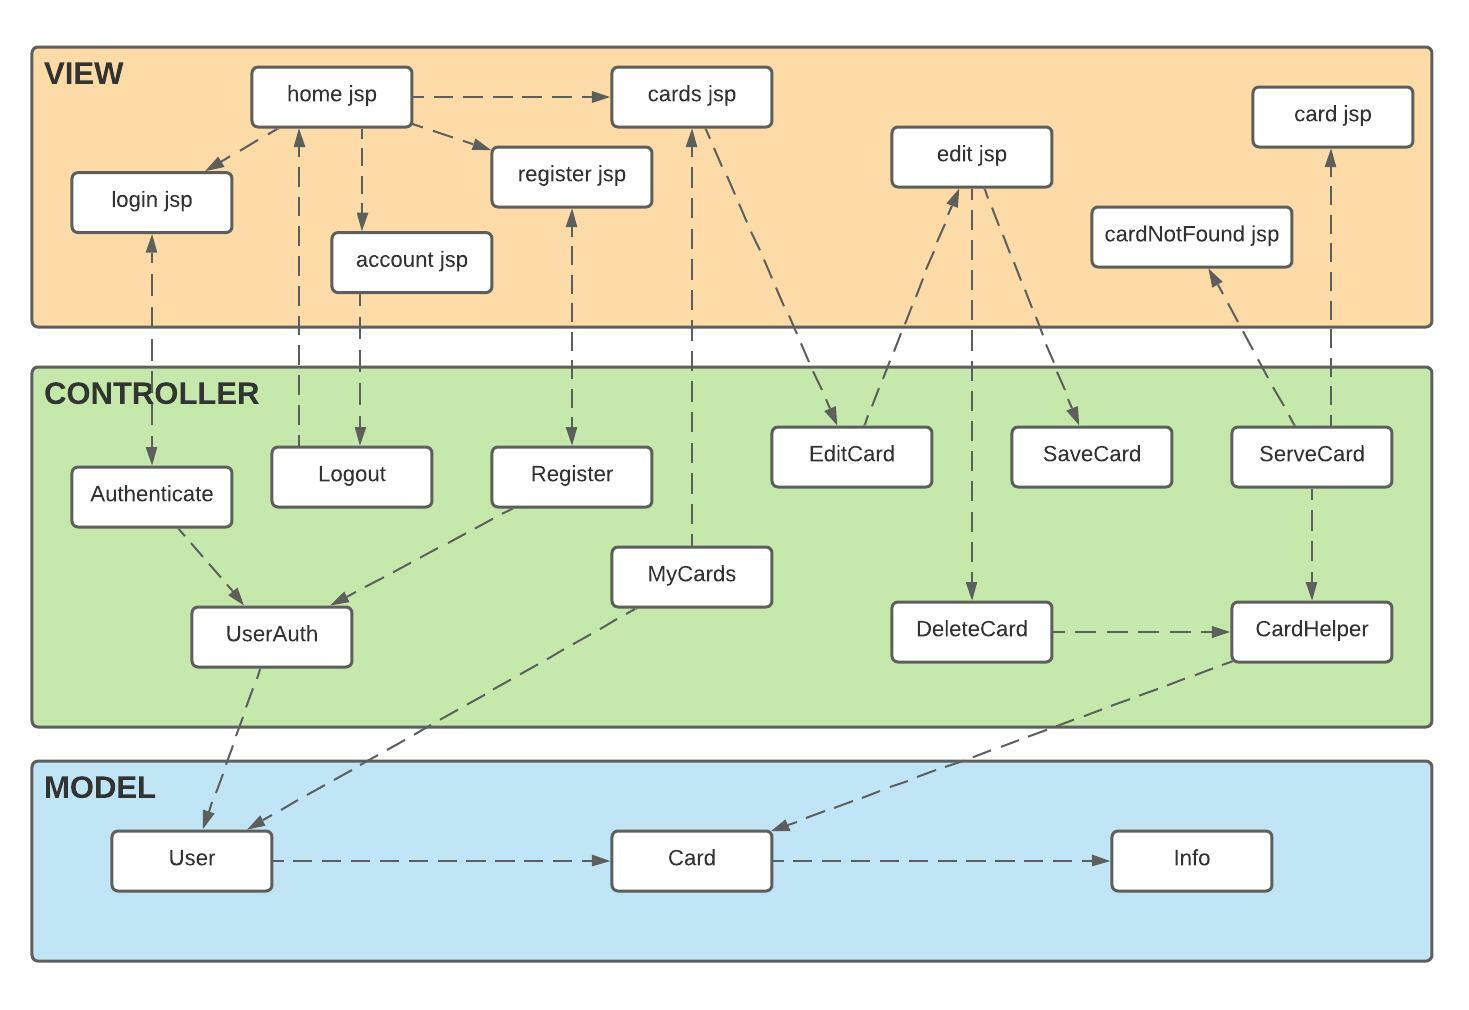
\includegraphics[width=0.55\paperwidth]{mvc_2.jpeg}}
	
	
	\item Above is an example of our Model View Controller. This diagram shows how we organized our login in order to neatly create our website. 
	The Model portion holds the more business layer of our application and this needs the Controller portion to help manage how the application works. 
	The controller is very important and helps bring everything together and makes sure it runs smoothly, while the View portion is mostly the presentation
	layer of our application and is what the user is seeing, thus containing the .jsp files. 

\end{enumerate}

\clearpage
\section{System Snapshot}
\begin{center}

	{\bf \Large Home Page}
	\makebox[\textwidth]{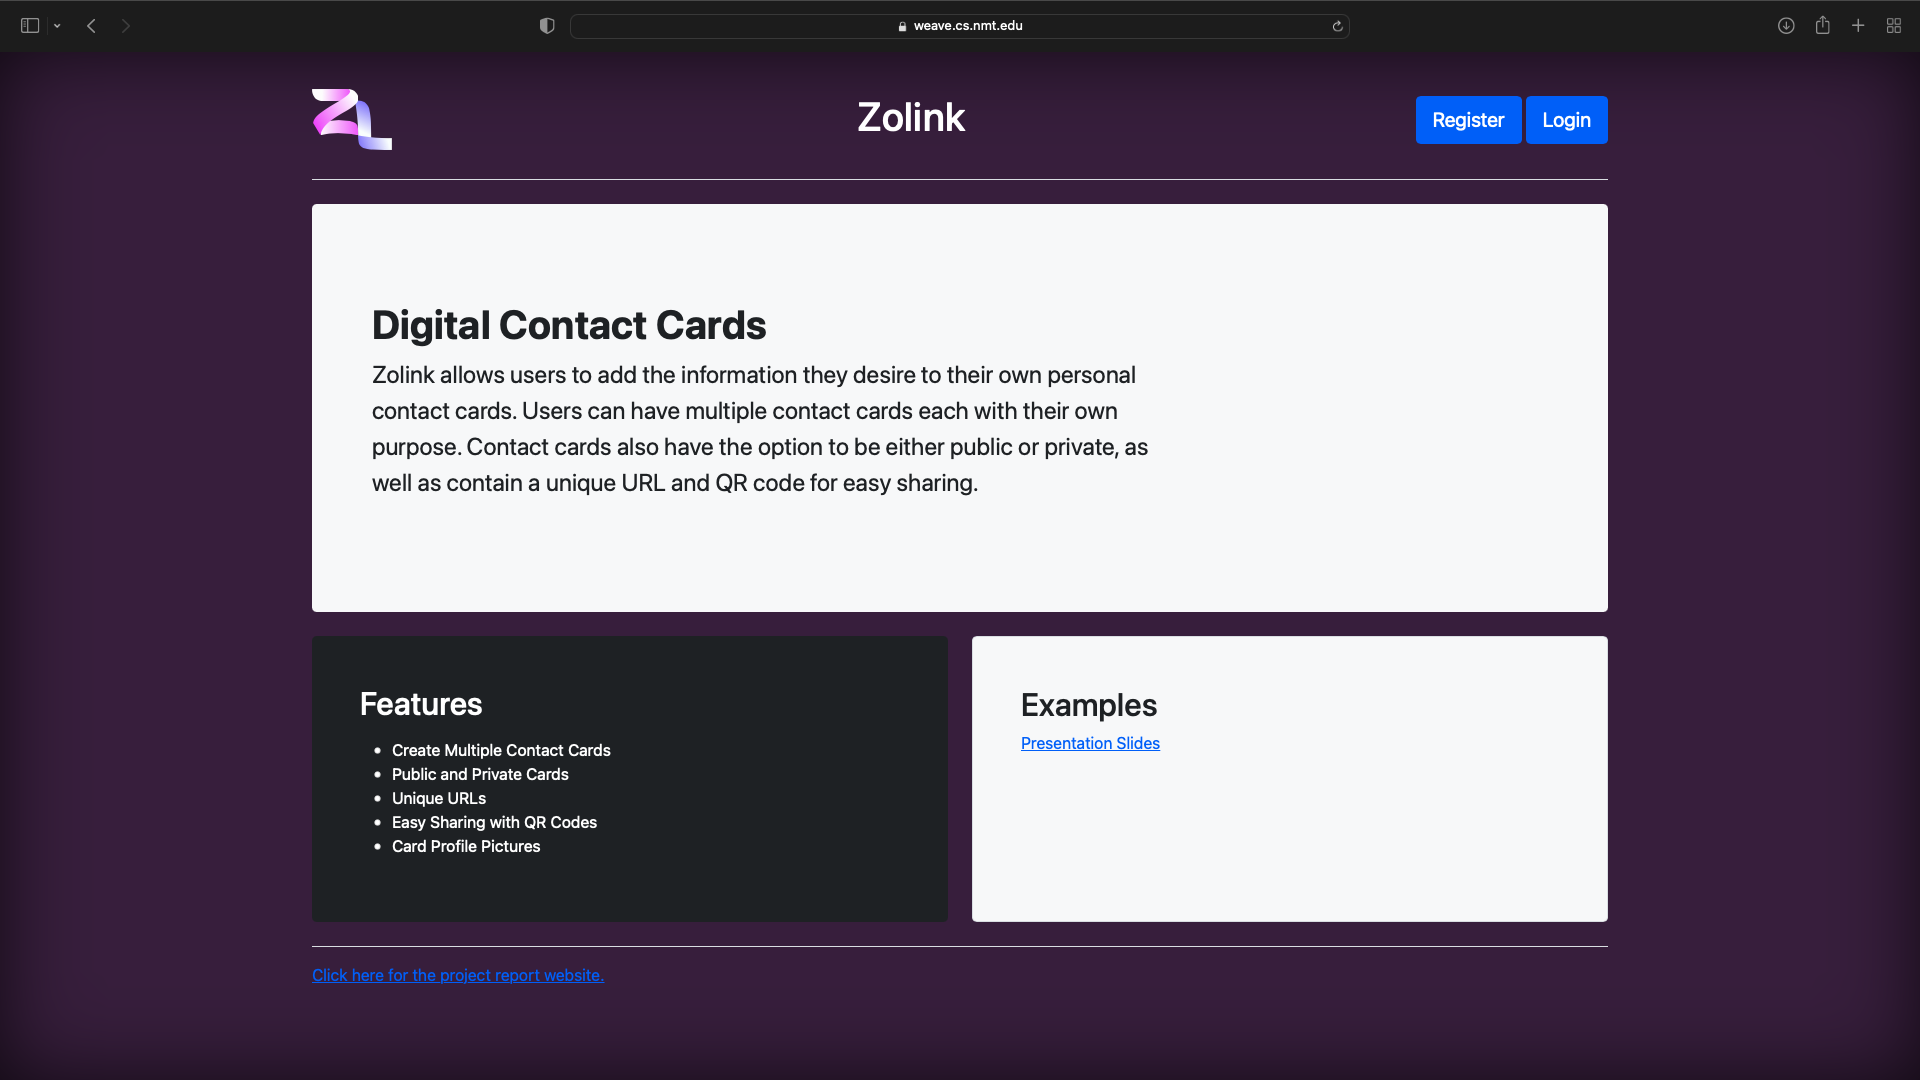
\includegraphics[width=0.90\paperwidth]{snapshot_images/home}}
	{\it This is our home page that explains what Zolink's purpose is.
		We hope to add an example of contact cards in the future. If the user already has an account with Zolink, they 
	can click login. If they would like to create an account they can click register. }
	
	
	\clearpage
	{\bf \Large Registration Page}
	\makebox[\textwidth]{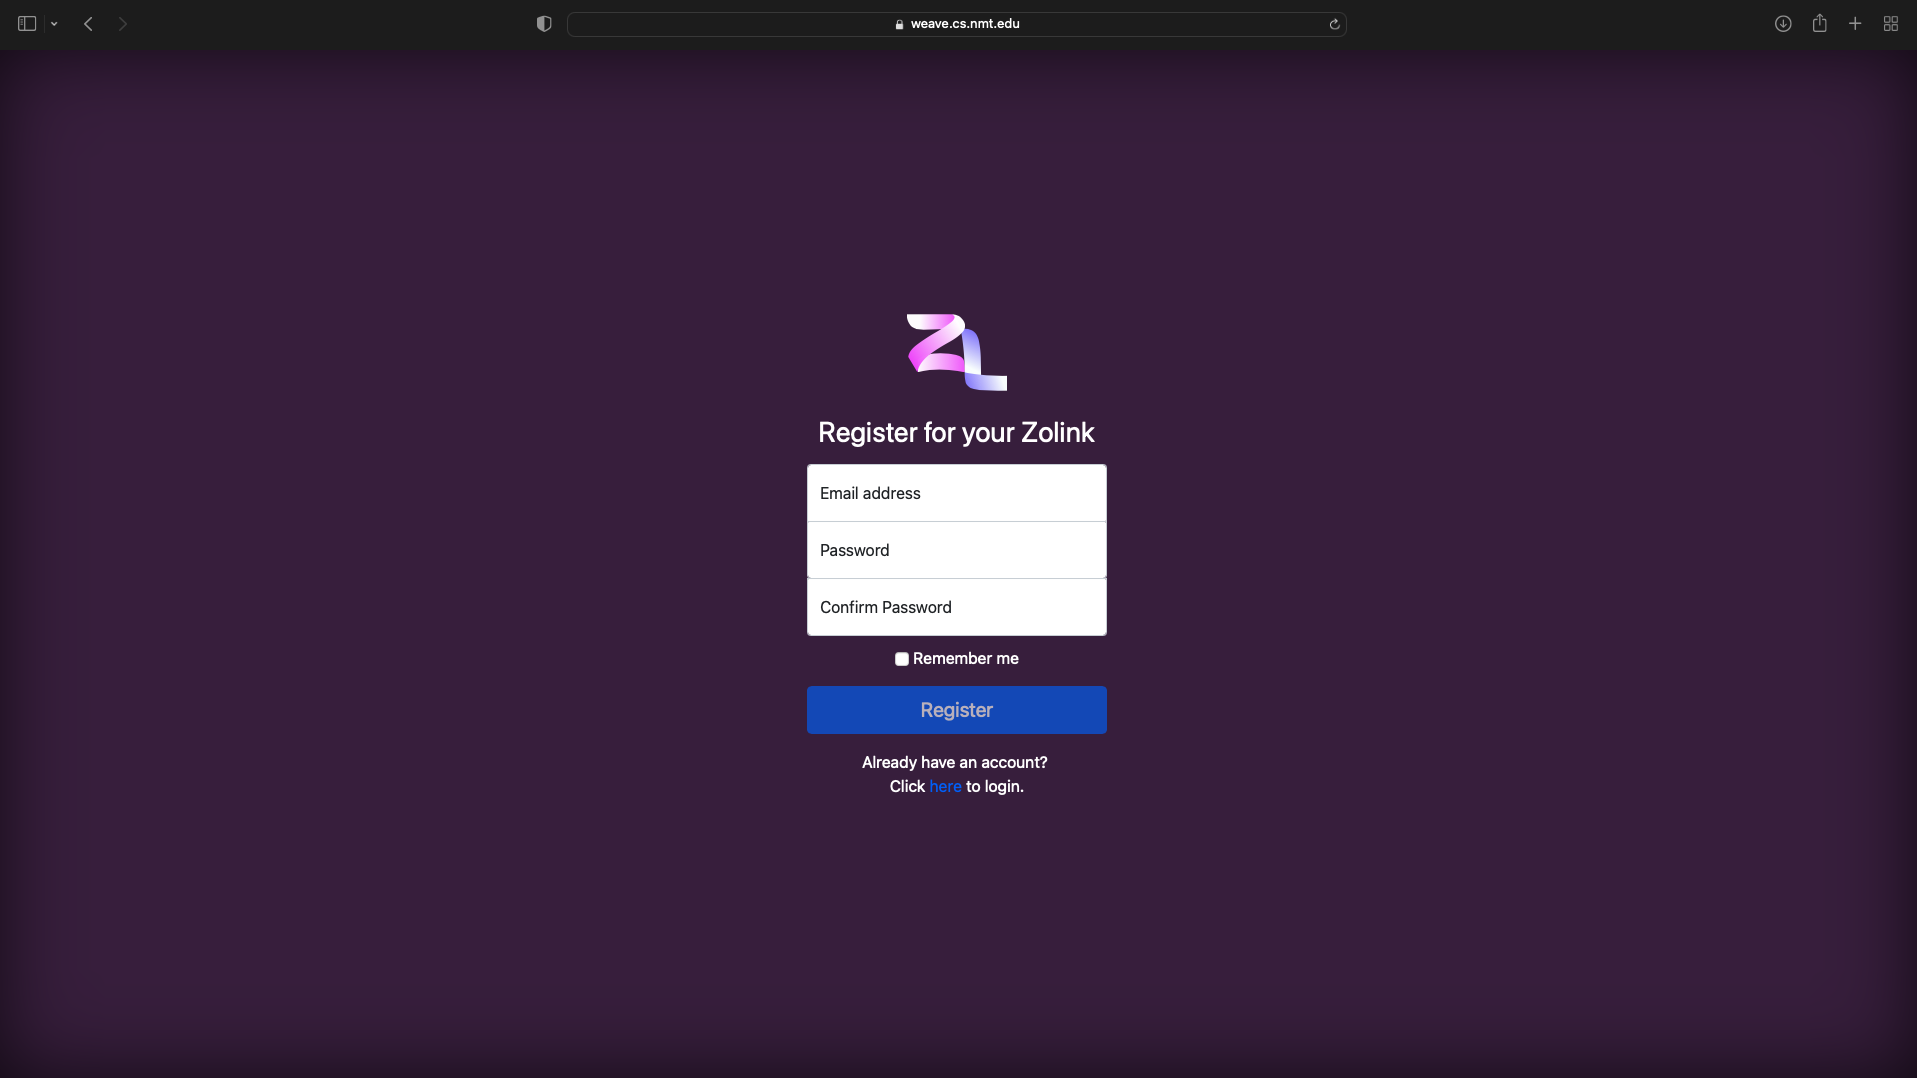
\includegraphics[width=0.98\paperwidth]{snapshot_images/register}}
	{\it If the user clicks "Register" on the home page, then they will be brought to this page. Here they can enter an 
	email address and a password. The password must be at least six characters. After they have filled out the forms they can 
	click "Register" to create their account. Note: if they are using an email that already has an account an error message will occur 
	informing the user that the email address is already in use.}

	\clearpage
	{\bf \Large Login Page}
	\makebox[\textwidth]{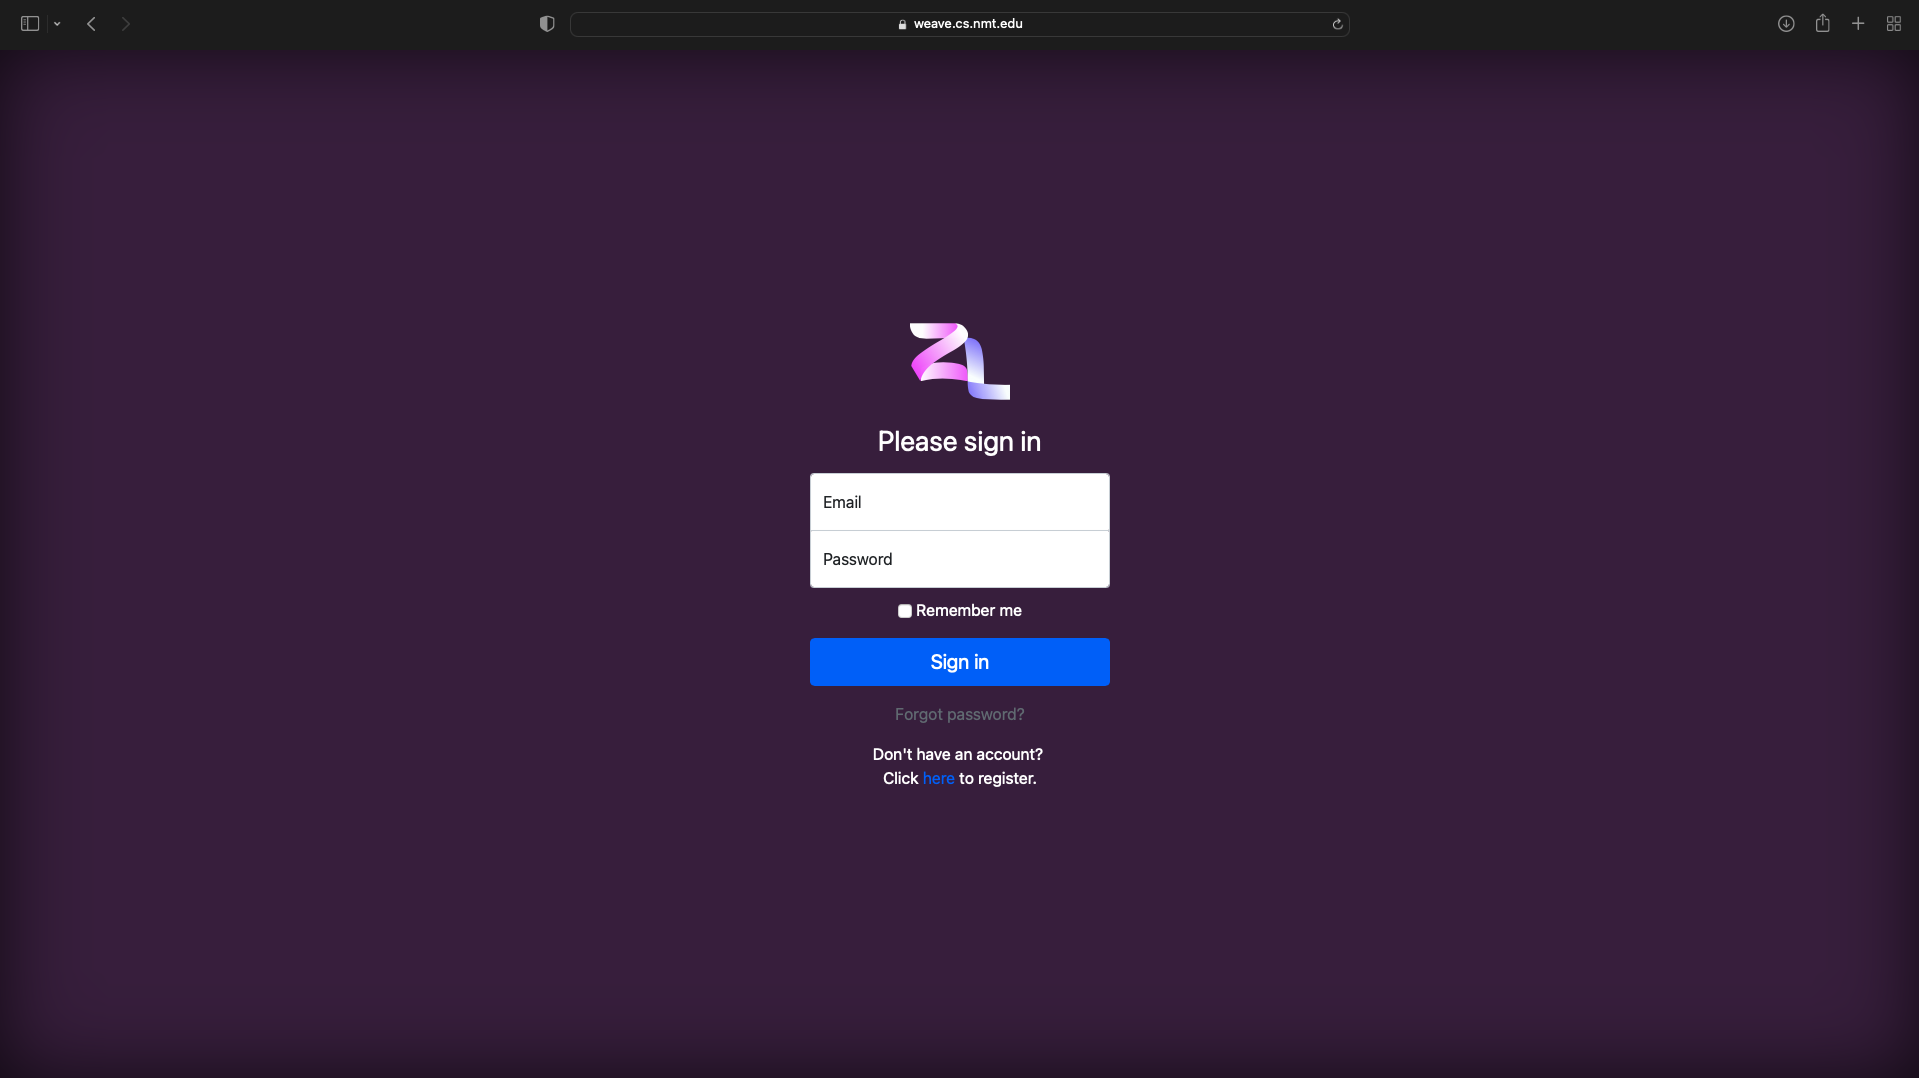
\includegraphics[width=0.98\paperwidth]{snapshot_images/login}}
	{\it If the user clicks "Login" on the home page, they will be brought to this page. Here they can enter their email and password 
	and press "Login" to enter their account. Note: If they enter the wrong password an error message will notify the user that their 
	password was wrong.}
	
		\clearpage
	{\bf \Large My Cards Page}
	\makebox[\textwidth]{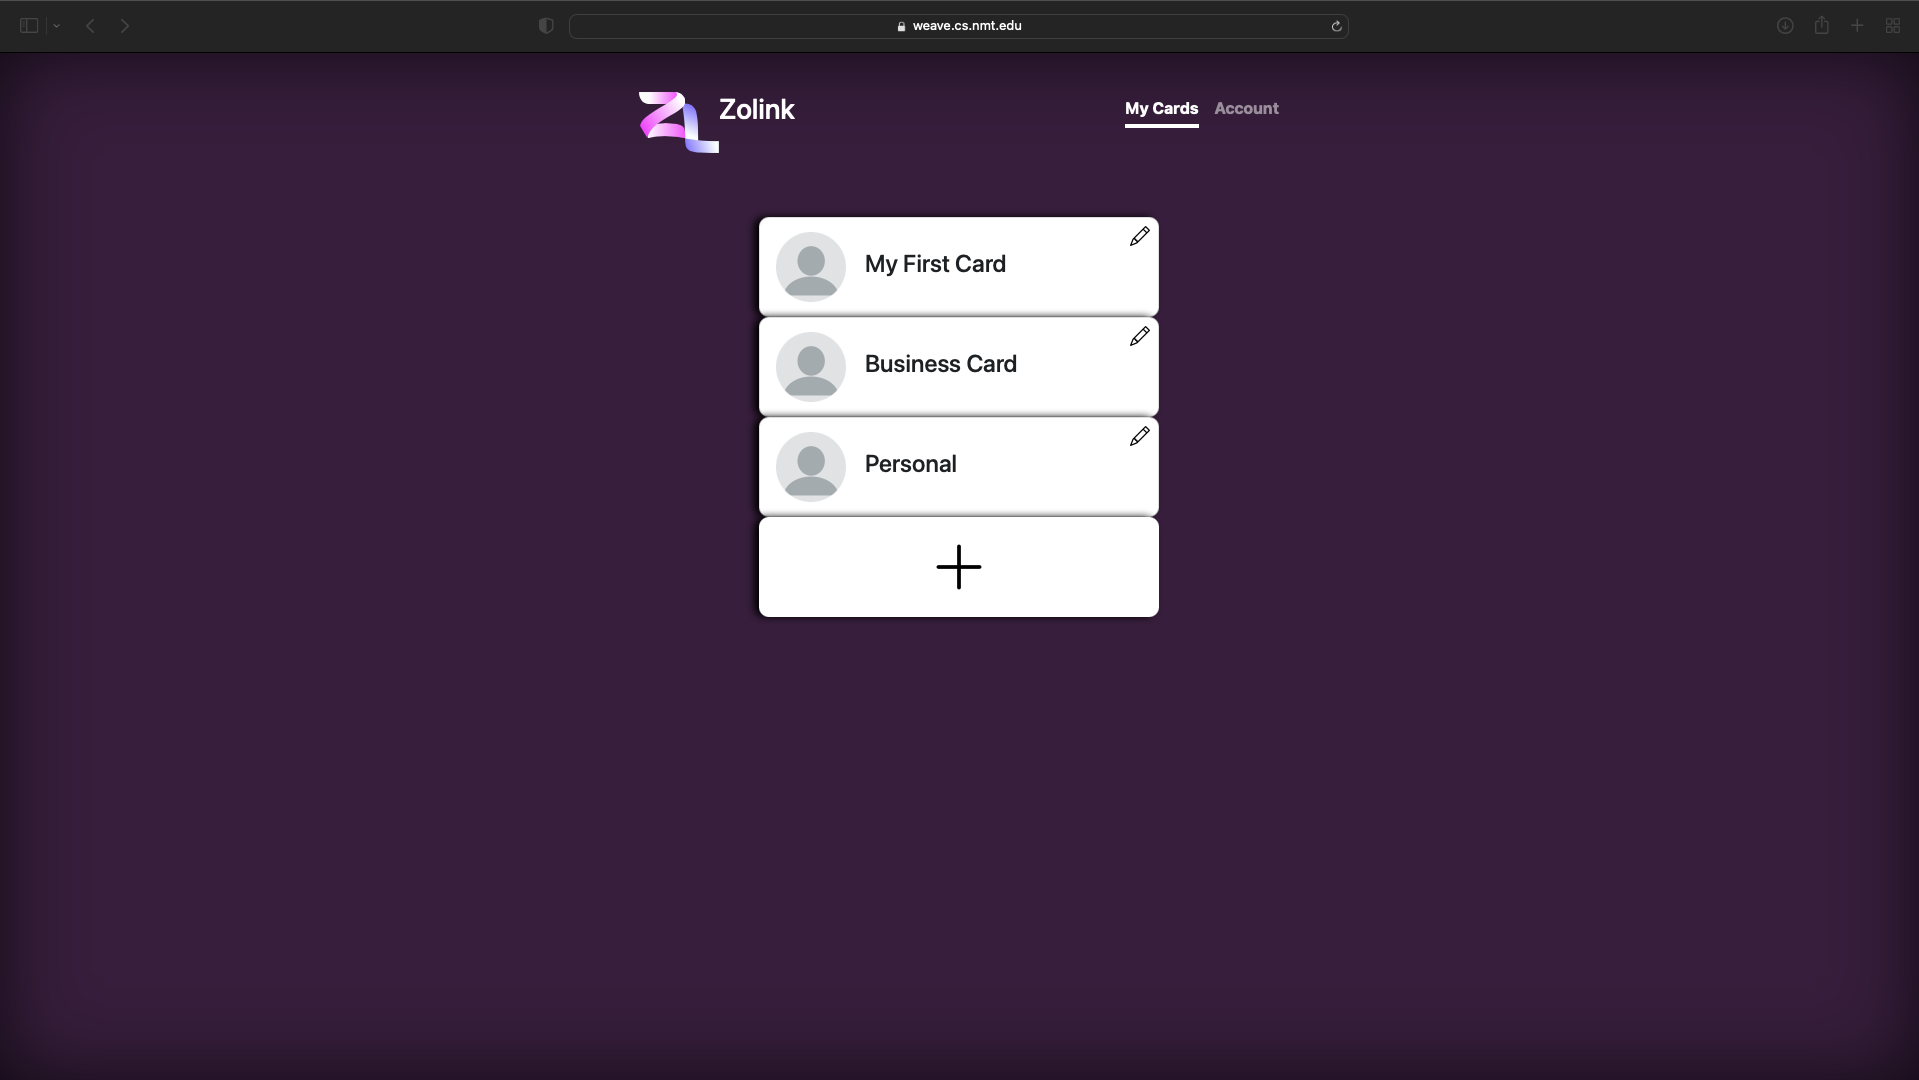
\includegraphics[width=0.98\paperwidth]{snapshot_images/myCards}}
	{\it After Logging in the user will be directed to the "My Cards" page. Here they can see all of their created cards, as well as choose to 
	edit one of their cards by pressing the pencil on the top right corner of the card, or to create a new card by pressing the Plus. If they would 
	like to view the card they can just click on the card they want to view. They can also view their account info by clicking the "Account" button
	in the top right corner.}
	
		\clearpage
	{\bf \Large New Card Page}
	\makebox[\textwidth]{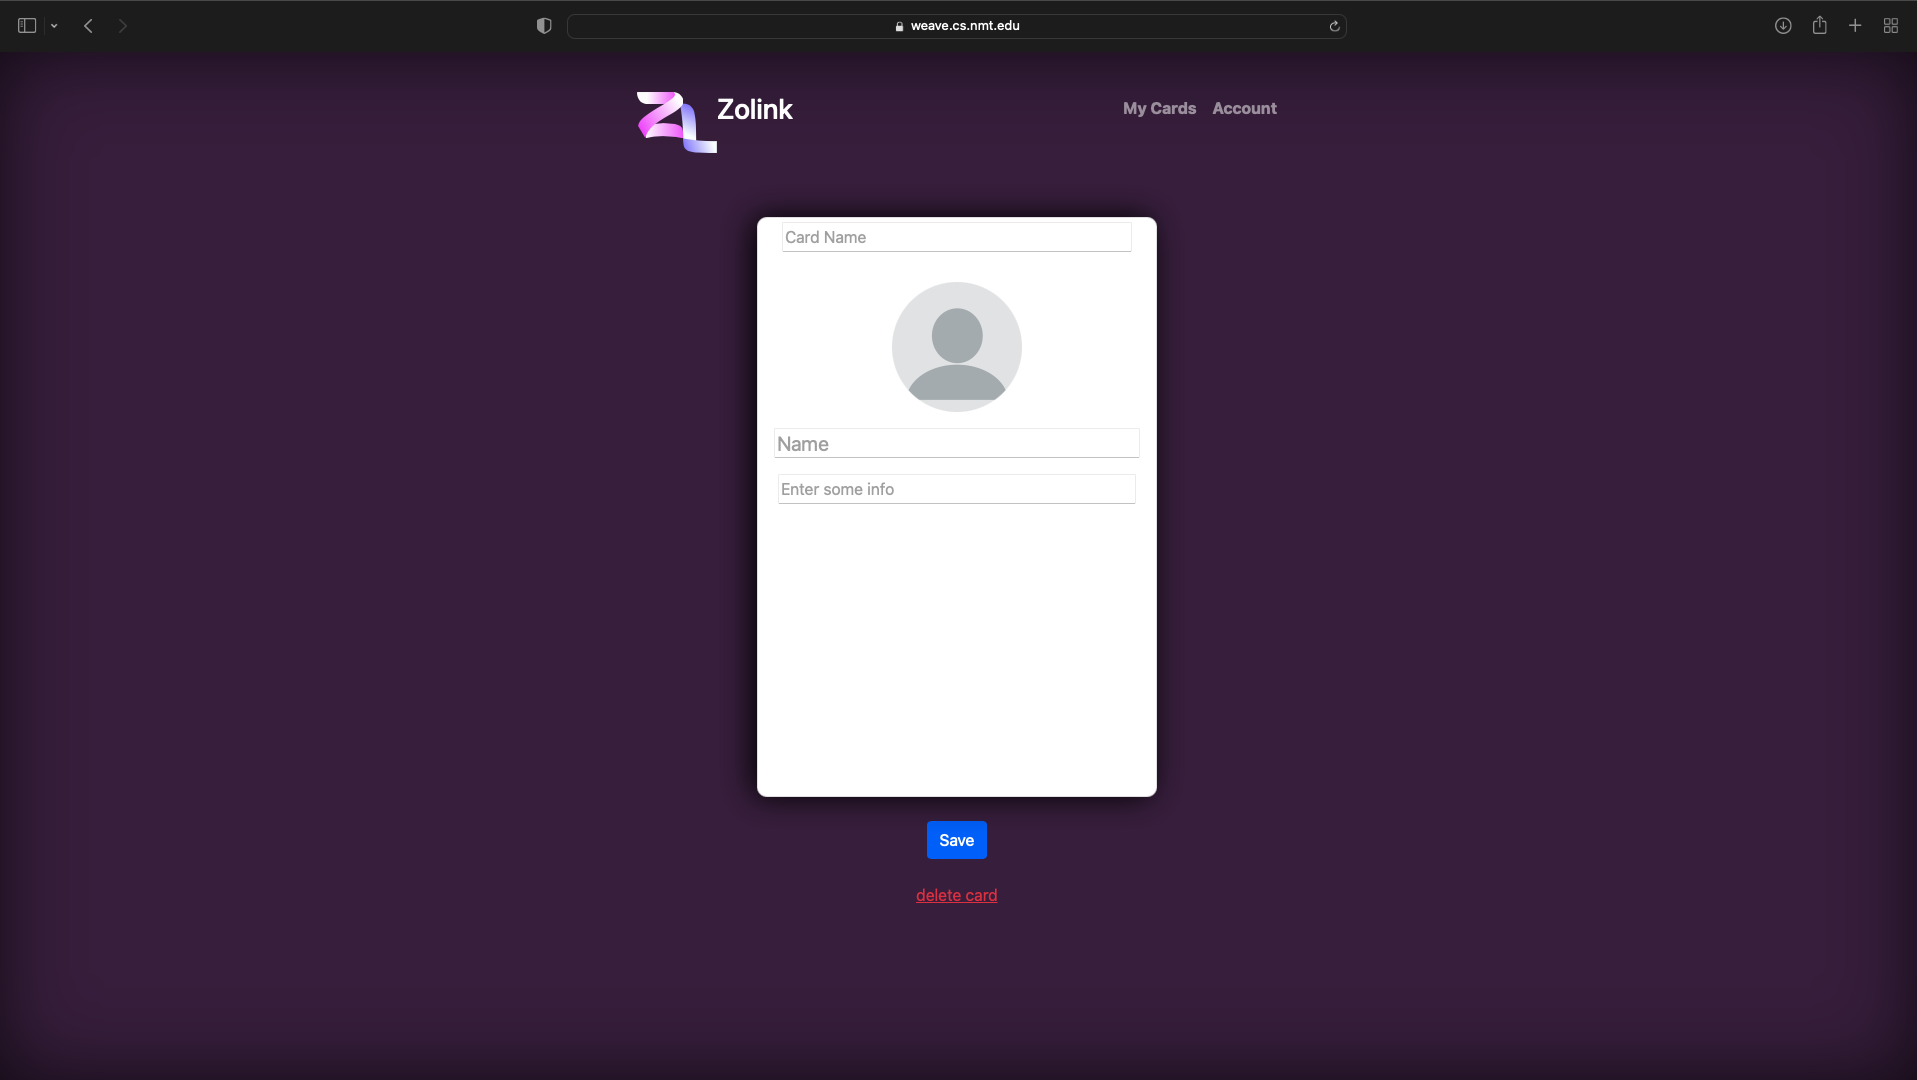
\includegraphics[width=0.98\paperwidth]{snapshot_images/newCard}}
	{\it If the user clicks on the PLUS they will be directed to the new card page, here they can create a new contact card, everytime one info field is 
	filled up a new field will pop up below, after they create their card they can save their card by pressing the "Save" button, or they can choose to 
	delete the card by pressing the "delete card" button.}
	
		\clearpage
	{\bf \Large Edit Card Page}
	\makebox[\textwidth]{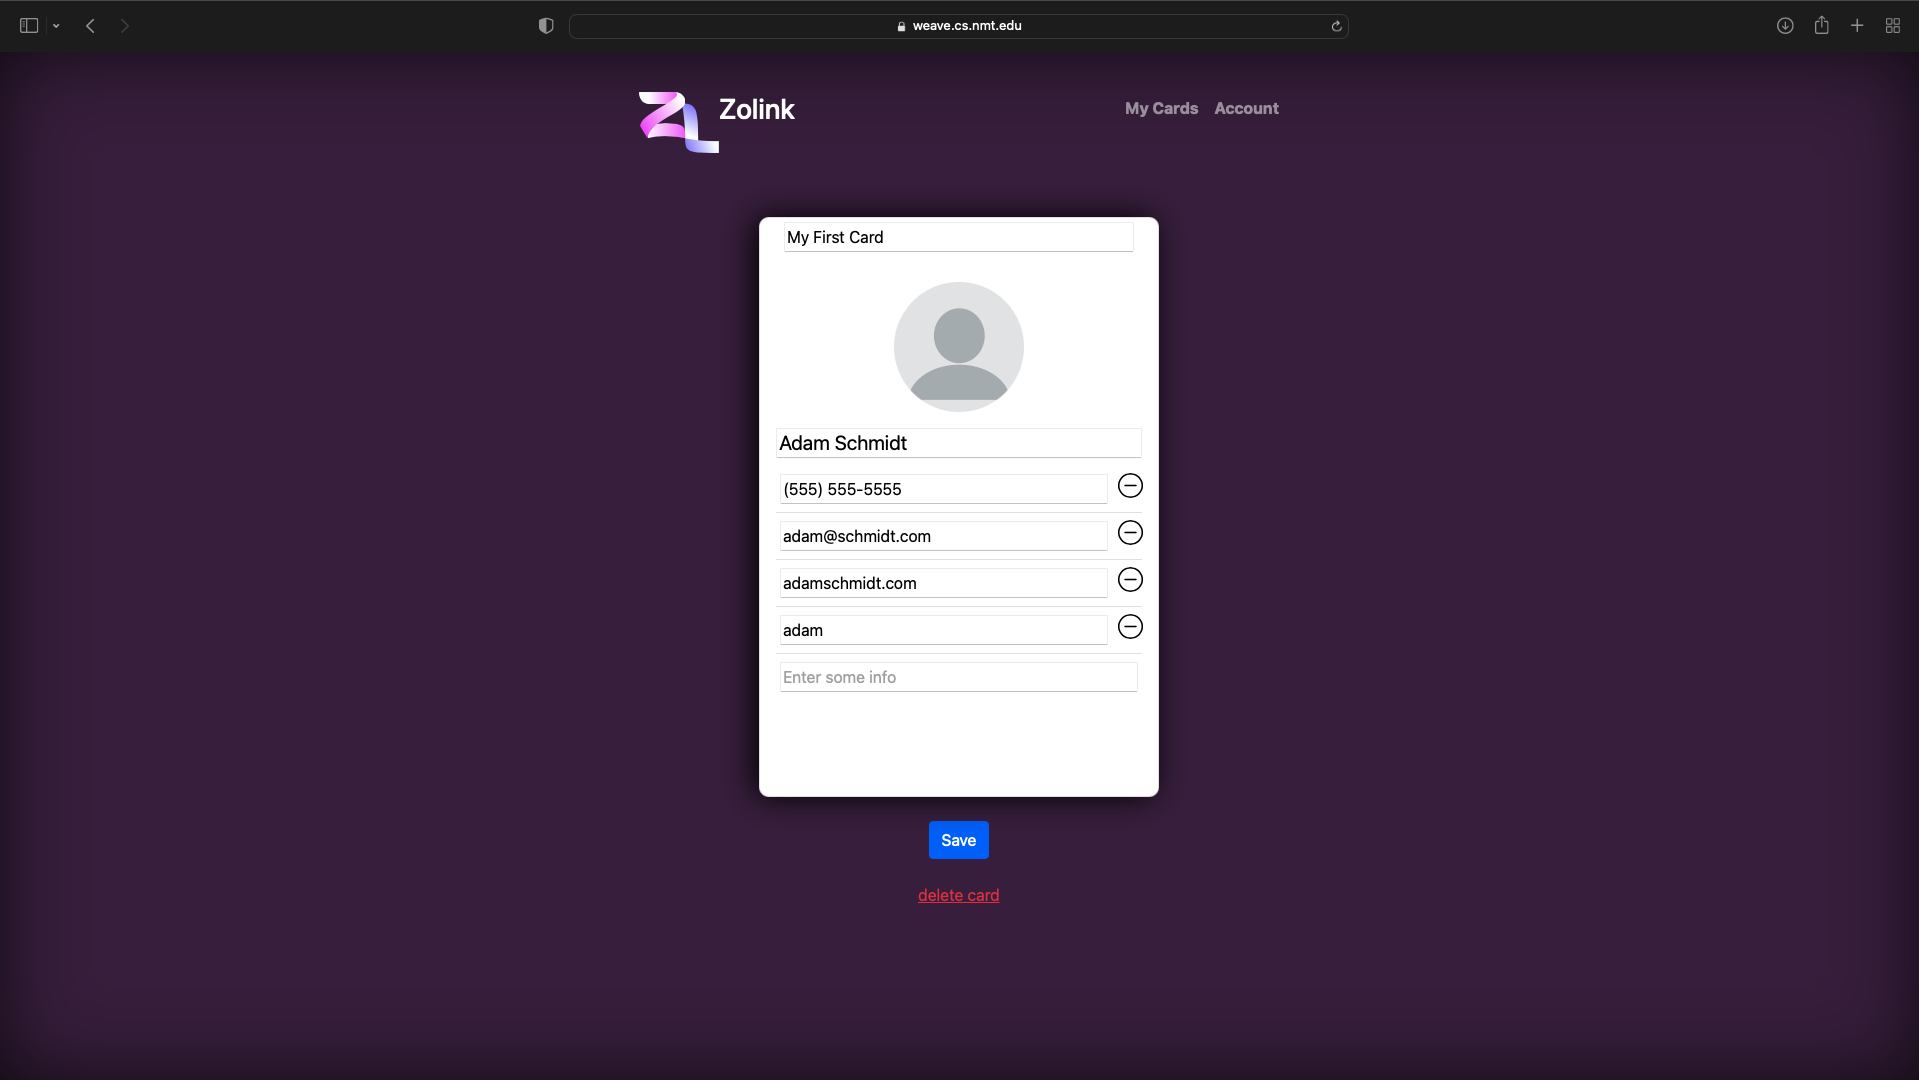
\includegraphics[width=0.98\paperwidth]{snapshot_images/cardEdit}}
	{\it If the user decides to edit a card and clicks on a card, for example this user clicked on the edit button on their card called "My First Card" 
	which brought the user
	to this page which will allow the user to edit that card. The user will be able to add more info to their card or take info off of their card by pressing the 
	minus next to one of the fields. The user can then save their card by pressing the "Save" button, or they can choose to 
	delete the card by pressing the "delete card" button.}
	
		\clearpage
	{\bf \Large Card View Page}
	\makebox[\textwidth]{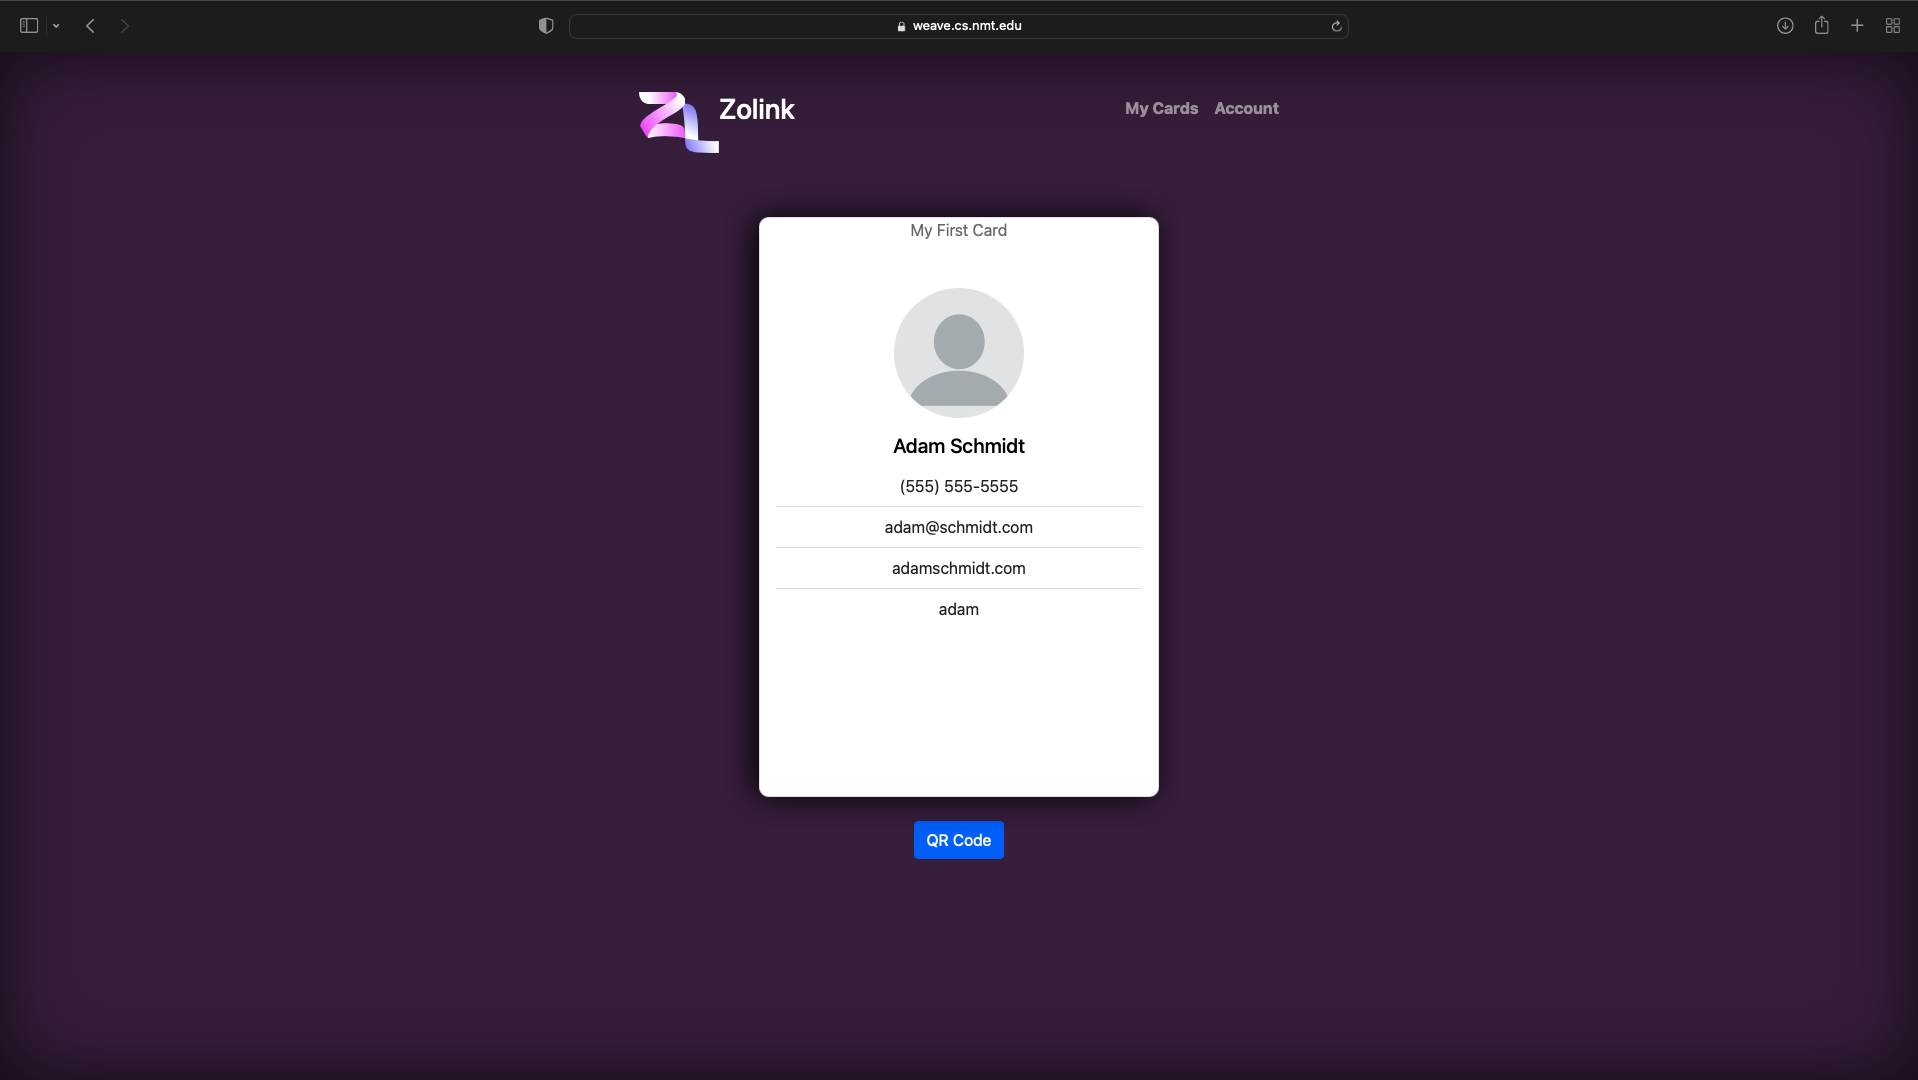
\includegraphics[width=0.98\paperwidth]{snapshot_images/exCardView}}
	{\it If the user wants to view one of their cards, they can click on the card name, for example this user clicked on their card called "My First Card" 
	which brough them to this page. Here you can view your card's info. You can share this card by giving someone your unique URL or QR code. The unique
	URL is found on the html and is the last four letters/numbers of the URL. To access the QR code you can just click the "QR Code" button on the bottom
	of the card.}

		\clearpage
	{\bf \Large Example Unique URL}
	\makebox[\textwidth]{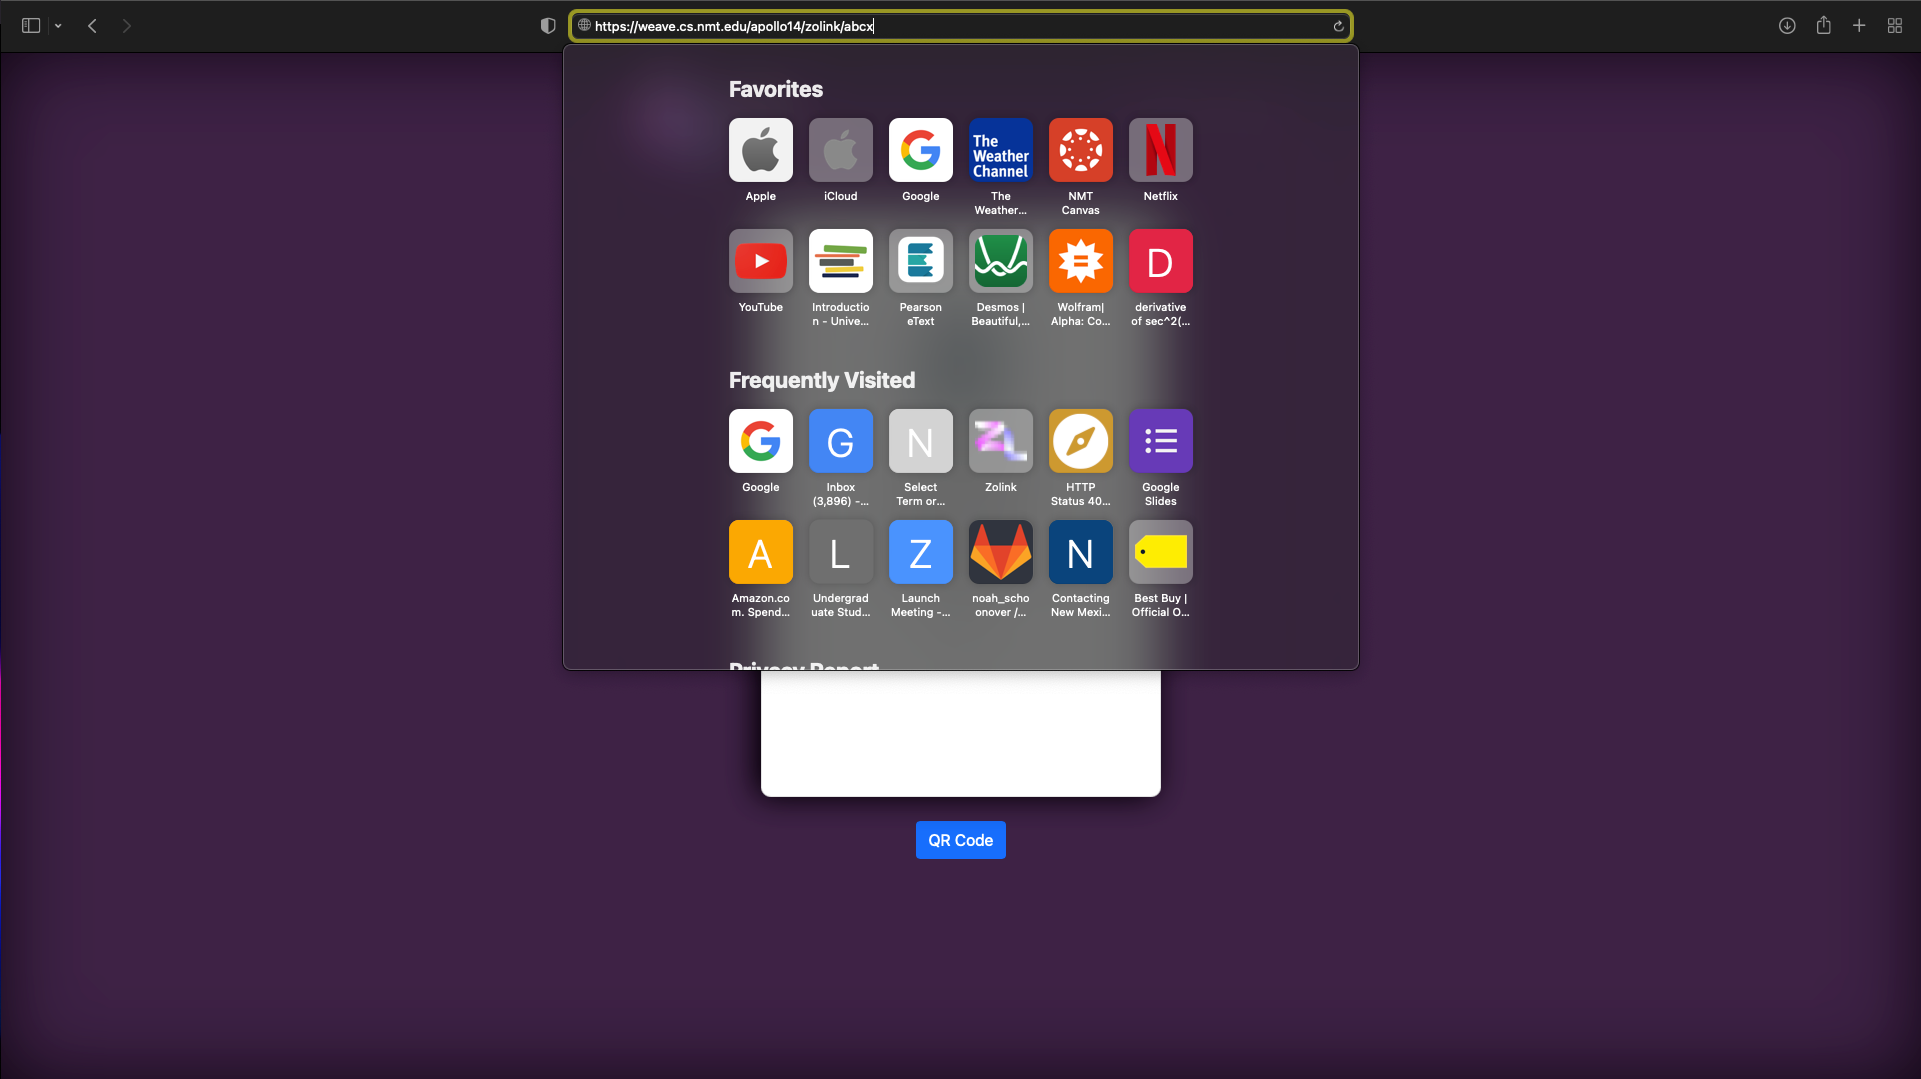
\includegraphics[width=0.98\paperwidth]{snapshot_images/exCardURL}}
	{\it Here you can see the Unique URL of this card, since it is the last four letters/numbers of the URL, this cards unique code will be "abcx". If you wanted
	to share your contact card so a friend could view it, they would just need to enter "zolink.me/abcx" into a browser, this will bring them to view your contact
	card.}
	
		\clearpage
	{\bf \Large Example Card QR Code Page}
	\makebox[\textwidth]{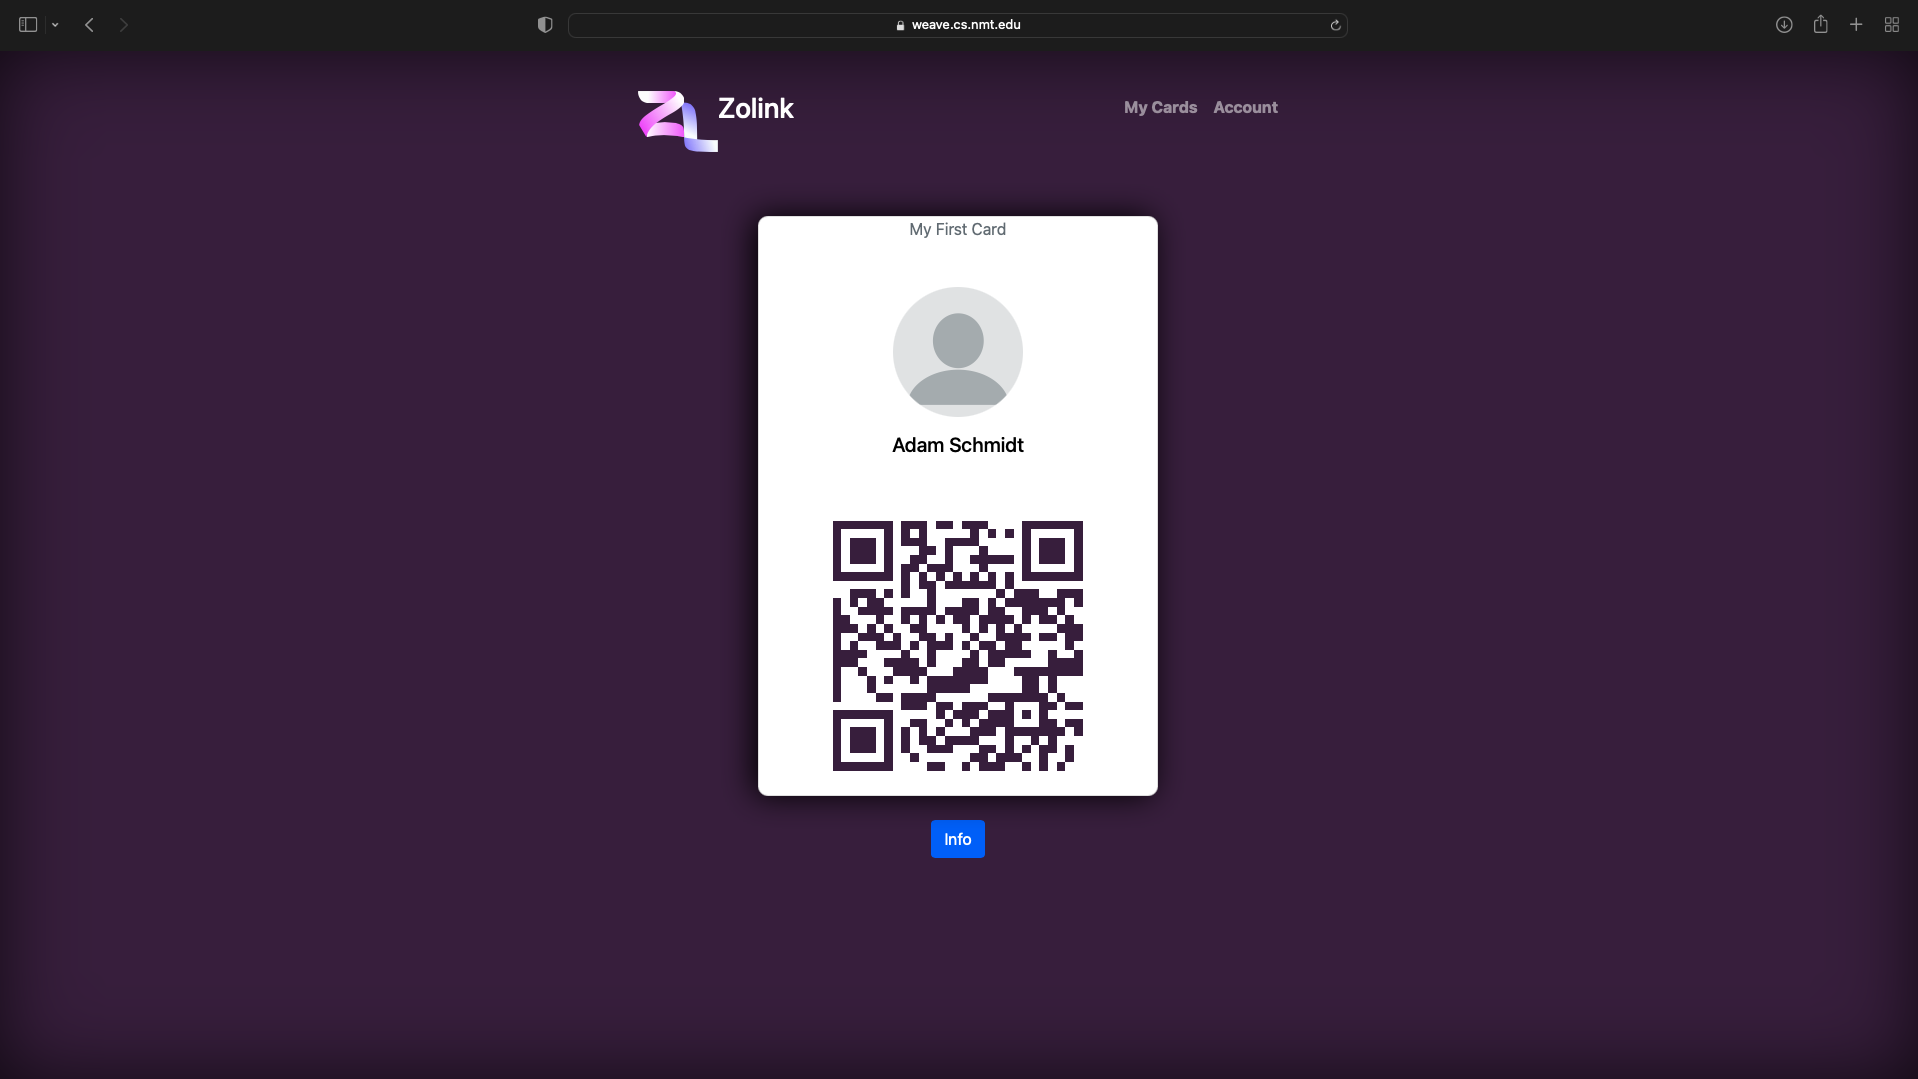
\includegraphics[width=0.98\paperwidth]{snapshot_images/exCardQR}}
	{\it If the user wanted to view/share their QR code, they could press the QR button on the bottom of the card which will flip their card and show the unique
	QR code that is on the back of their card (as shown in the example above).}
	
		\clearpage
	{\bf \Large Account Page}
	\makebox[\textwidth]{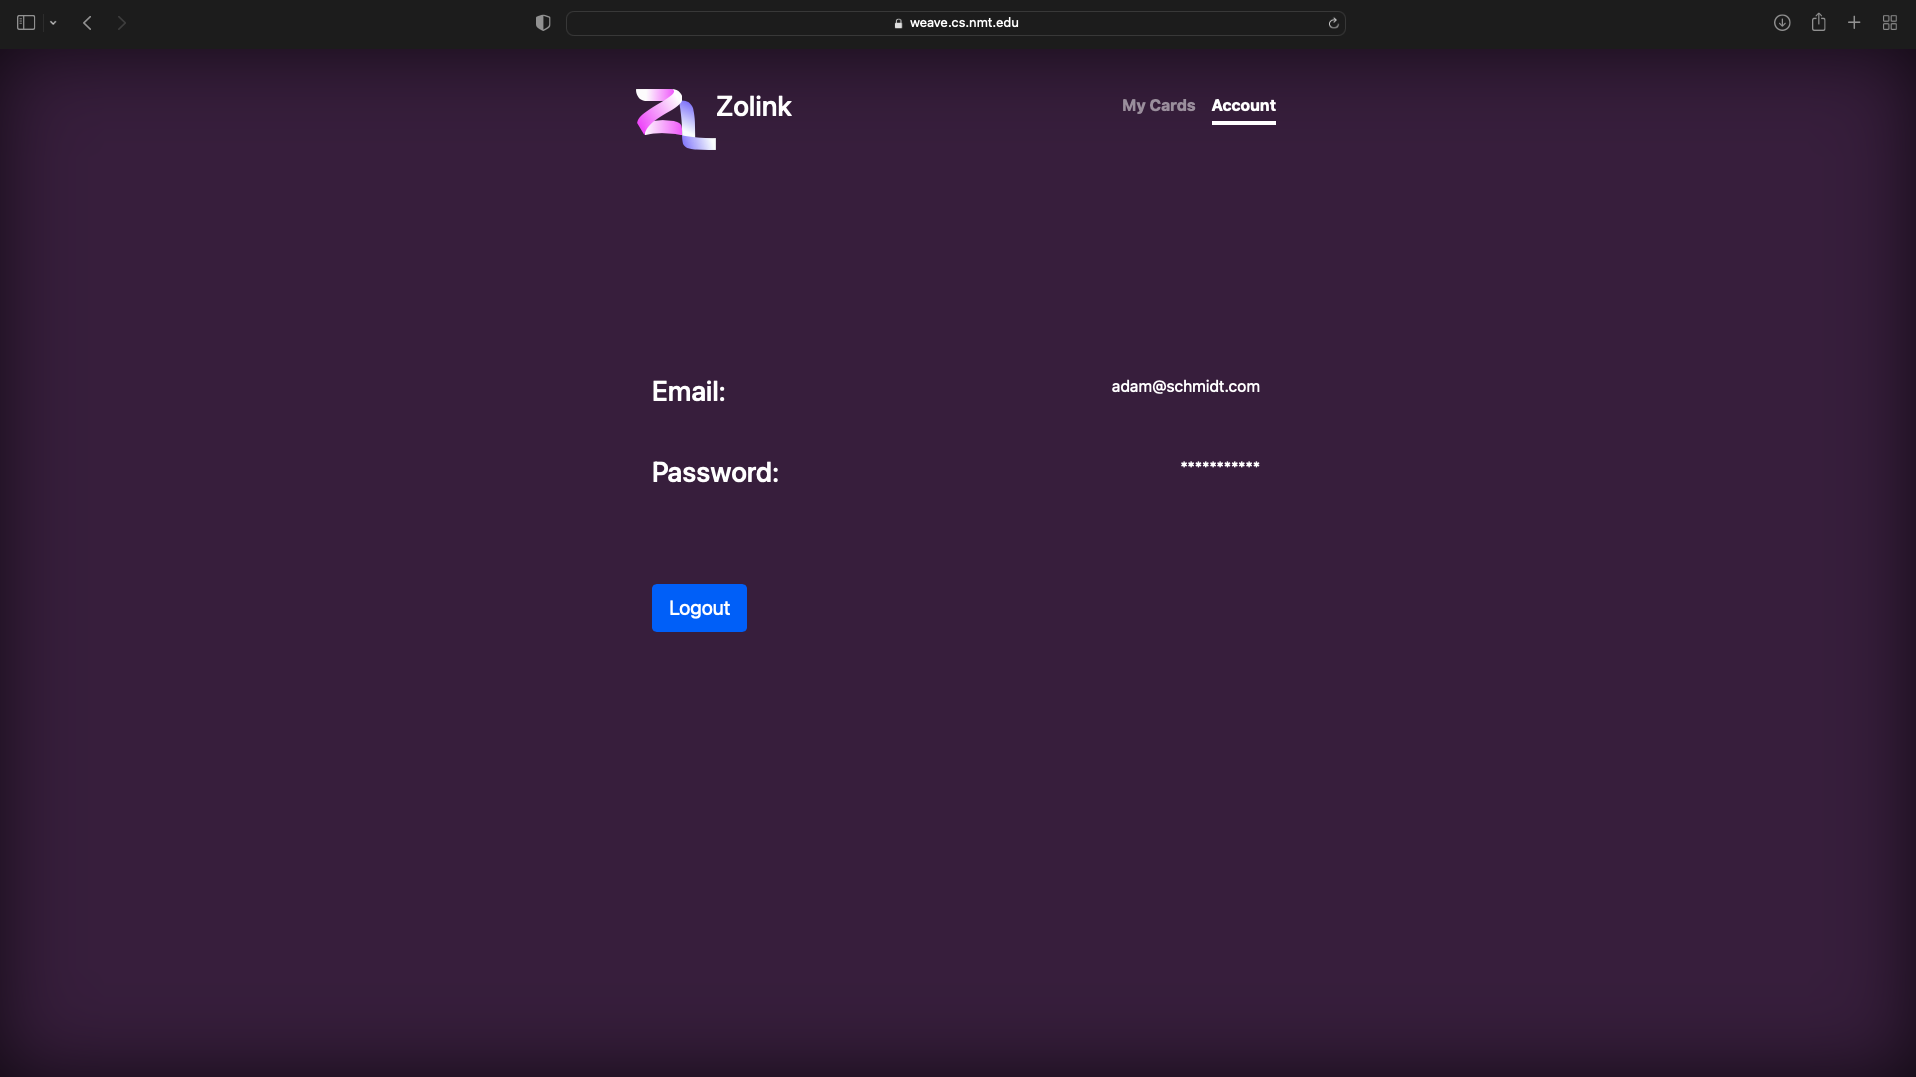
\includegraphics[width=0.98\paperwidth]{snapshot_images/account}}
	{\it If the user decides to view/logout of their account, they can click on the "Account" button on the top right of the page, here they can view their account
	info as well as logout by clicking the "Logout" button.}

\end{center}

\clearpage
\section{Conclusion}
\begin{enumerate}[7.a.]
	
	\item {\bf What We Accomplished:} 
	
	During this project we have learned a great deal about what goes into web programming. Through different steps throughout the course we have been able
	to learn and implement our knowledge on Servlets and XML services to create our website. We have learned the importance of creating a prototype to work
	off of; as well as how necessary the smaller steps are to creating and completing a well designed website. Our final project follows our initial storyboard idea
	very closely with very few detials left out. Besides some small things we would like to add to our site in the future, our final project is complete and runs 
	perfectly on the CS weave server. 
	
	\item {\bf What We Want to Add in the Future:}
	
	A few details that we would like to add in the future would be to allow users to add their profile pictures to their cards. We also want to implement private
	cards so people can decide who will be able to view their cards. We want to add a few example pictures of cards to the home page so that people can 
	see what kind of cards can be made with Zolink. Another improvement would be to implement dynamic info types so that when users add for example
	and Instigram handle, then the card would show the Instagram picture next to the handle. 
	
	
\end{enumerate}

%============================================================================
\end{document}
%============================================================================
